% ==============================================================================
% PART 2: CHAPTER 3 (MATHEMATICAL FORMULATION) \& CHAPTER 4 (SYSTEM DESIGN)
% ==============================================================================

\chapter{MATHEMATICAL FORMULATION}

\section{Overview}
The Explainable Intelligence Engine (XIE) integrated with the 4-Domain Model Context Protocol (MCP) Agentic AI forms a mathematically rigorous, closed-loop Site Reliability Engineering (SRE) and Active Cyber-Defense framework for our 5-plane bare-metal OpenStack, Kubernetes 5G Core, USRP B210 SDR, and Dual-GPU data center. Rather than relying on heuristic threshold rules or unconstrained LLM prompting, the system continuously ingests a 54-feature cross-layer telemetry vector $\mathbf{x}(t) \in \mathbb{R}^{54}$ every $\Delta t = 5\text{ s}$, capturing both spatial topological dependencies across physical and virtualized planes and temporal state dynamics over a rolling window $W = 15$.

To guarantee both sub-second anomaly detection and $>98\%$ upstream root-cause attribution accuracy during cascading outages, our mathematical formulation unifies seven complementary components:
\begin{enumerate}
    \item \textbf{Rolling Z-Score Standardization} ($\mathbf{z}(t) \in \mathbb{R}^{54}$) for scale-invariant anomaly gating across heterogeneous physical units (dB, Mbps, \%, GFLOPS, packet counts);
    \item \textbf{Balanced Random Forest Ensemble Classification} ($P_{\text{RF}}(y \mid \mathbf{x}(t))$) with inverse class-frequency weighting to handle rare fault states;
    \item \textbf{Vector Autoregression $\text{VAR}(L)$ and Granger Causality F-Tests} to statistically discover directed temporal fault-propagation edges $(i \to j)$ across planes;
    \item \textbf{Causal Edge Reversal ($G_{\text{rev}}$) and Personalized PageRank (PPR)} ($\boldsymbol{\pi} = (1-\alpha)(\mathbf{I}-\alpha\mathbf{P})^{-1}\mathbf{v}$) to walk \textit{upstream} against the direction of symptom cascading and isolate the true root-cause subsystem $i^*$;
    \item \textbf{Spatio-Temporal Graph Neural Network (ST-GNN) and LSTM Gate Dynamics} to capture non-linear message passing and multi-tick temporal memory;
    \item \textbf{ChromaDB HNSW Vector Cosine Similarity Recall} for sub-15ms zero-shot recognition of recurring operational fault episodes; and
    \item \textbf{Dual-GPU Autoregressive LLM Conditioning (\texttt{qwen3:14b})} for asynchronous post-mortem synthesis.
\end{enumerate}

\section{Objective Function}
The overarching mathematical objective of the autonomous Agentic AI recovery framework is to minimize the expected \textbf{Mean Time To Recovery (MTTR)} across the probability distribution of all operational infrastructure and security faults $f \sim \mathcal{F}$, while simultaneously maximizing diagnostic root-cause precision:
\begin{equation}
\min_{\Theta, \Pi} \; \mathbb{E}_{f \sim \mathcal{F}} \left[ \text{MTTR}(f; \Theta, \Pi) \right]
\label{eq:obj_main}
\end{equation}

\noindent\textbf{Term Elaboration:}
\begin{itemize}
    \item $\min_{\Theta, \Pi}$: Denotes the joint optimization problem over the learnable mathematical critic parameters $\Theta = \{ \mathbf{W}_{\text{RF}}, \mathbf{\Phi}_{\text{VAR}}, \mathbf{W}_{\text{GCN}}, \mathbf{W}_{\text{LSTM}}, \alpha, \tau \}$ and the deterministic MCP agentic remediation policy rules $\Pi : \mathcal{S} \to \mathcal{A}$.
    \item $\mathbb{E}_{f \sim \mathcal{F}}[\cdot]$: Denotes the statistical expectation over the empirical distribution of cross-layer faults $\mathcal{F}$ (comprising SDN OVS Geneve drops, Open5GS UPF crashes, compute host CPU saturation, USRP B210 RF attenuation, and Wazuh SSH brute-force attacks).
    \item $\text{MTTR}(f; \Theta, \Pi)$: Represents the total elapsed wall-clock downtime (in seconds) from the physical onset of fault $f$ at $t_0$ until full end-to-end SLA verification at $t_{\text{recovered}}$.
\end{itemize}

We mathematically decompose $\text{MTTR}(f)$ into four sequential, non-overlapping temporal phases:
\begin{equation}
\text{MTTR}(f) = T_{\text{detect}}(\Theta) + T_{\text{rca}}(\Theta) + T_{\text{remediate}}(\Pi) + T_{\text{verify}}(\Pi)
\label{eq:mttr_decomp}
\end{equation}

\noindent\textbf{Term Elaboration:}
\begin{itemize}
    \item $T_{\text{detect}}(\Theta)$: Time elapsed between physical fault injection $t_0$ and anomaly gating via rolling Z-score and Balanced Random Forest inference (empirically $\approx 0.08\text{ s}$ compute latency after telemetry arrival, median $\text{MTTD} = 0.42\text{ s}$).
    \item $T_{\text{rca}}(\Theta)$: Time required to isolate the root-cause node $i^*$, either via Fast-Path ChromaDB HNSW vector recall ($\approx 0.012\text{ s}$) or Slow-Path $\text{VAR}(2)$ + Reversed-DAG PPR power iteration ($\approx 0.40\text{ s}$).
    \item $T_{\text{remediate}}(\Pi)$: Execution duration of the surgical MCP tool call dispatched to \texttt{mcp-dcops}, \texttt{mcp-devops}, or \texttt{mcp-secops} ($\approx 1.37\text{ s}$).
    \item $T_{\text{verify}}(\Pi)$: Post-action telemetry probe verification confirming that all 54 Z-scores have returned to $|z_i| < 2.0$ and application HTTP/GTP-U endpoints return 200 OK ($\approx 0.46\text{ s}$). Note that Qwen3-14B report synthesis ($T_{\text{LLM}}$) is decoupled asynchronously and therefore adds $0\text{ s}$ to data-plane $\text{MTTR}(f)$.
\end{itemize}

To train and calibrate the mathematical critic parameters $\Theta$ and policy $\Pi$, we minimize a coupled multi-objective loss function $\mathcal{L}_{\text{total}}(\Theta, \Pi)$:
\begin{equation}
\mathcal{L}_{\text{total}}(\Theta, \Pi) = \mathcal{L}_{\text{CE}}(\Theta) + \lambda_1 \mathcal{L}_{\text{DAG}}(\mathbf{A}) + \lambda_2 \mathcal{L}_{\text{SLA}}(\Pi) + \lambda_3 \|\Theta\|_2^2
\label{eq:total_loss}
\end{equation}
where individual loss components are defined as follows:
\begin{align}
\mathcal{L}_{\text{CE}}(\Theta) &= -\frac{1}{N_b} \sum_{n=1}^{N_b} \sum_{c=1}^{C} w_c \, y_{n,c} \log \hat{p}_{n,c}(\Theta) \label{eq:loss_ce} \\
\mathcal{L}_{\text{DAG}}(\mathbf{A}) &= \text{Tr}\left( e^{\mathbf{A} \odot \mathbf{A}} \right) - M + \gamma \|\mathbf{A}\|_1 \label{eq:loss_dag} \\
\mathcal{L}_{\text{SLA}}(\Pi) &= \sum_{m=1}^{M} \max\left( 0, \; |z_m(t_0 + \Delta t_{\text{exec}})| - z_{\text{SLA}} \right)^2 \label{eq:loss_sla}
\end{align}

\noindent\textbf{Defense Intuition:} Equation (\ref{eq:loss_ce}) is the class-balanced cross-entropy loss across $C=5$ operational states with inverse-frequency weight $w_c = \frac{N}{C \cdot N_c}$. Equation (\ref{eq:loss_dag}) enforces sparsity ($\|\mathbf{A}\|_1$) and acyclicity ($\text{Tr}(e^{\mathbf{A}\odot\mathbf{A}}) - M = 0$) on the discovered causal graph $\mathbf{A}$, preventing circular blame loops. Equation (\ref{eq:loss_sla}) penalizes any remediation policy $\Pi$ that fails to bring all standardized telemetry metrics below the healthy threshold $z_{\text{SLA}} = 2.0$ immediately after action execution.

\section{System Constraints Affecting Objective Functions}
The optimization of Equations (\ref{eq:obj_main})--(\ref{eq:total_loss}) is subject to strict physical hardware, network protocol, and operational safety constraints imposed by our bare-metal telco-cloud environment:

\subsection*{1. Topological, Hardware \& SDN Capacity Constraints}
\begin{align}
\sum_{v \in \mathcal{V}_{\text{host}(h)}} \text{Mem}(v) + \text{Mem}_{\text{AI}}(h) &\le \text{Mem}_{\text{max}}(h) \quad \forall h \in \{\text{Dell R760xs}, \text{PC1}, \text{PC2}\} \label{eq:const_mem} \\
\text{VRAM}_{\text{tensor}}(g) &\le 4096\text{ MB} \quad \forall g \in \{\text{GPU}_0 (\texttt{10.10.10.4}), \text{GPU}_1 (\texttt{10.10.10.5})\} \label{eq:const_vram} \\
\text{MTU}(\texttt{ovn0-compu-}k) + 50\text{ B (Geneve Header)} &\le \text{MTU}_{\text{phys}}(\texttt{eno12399}) = 1500\text{ B} \label{eq:const_mtu} \\
\sum_{h \in \text{Cluster}} \mathbb{I}\left( \text{MySQL\_Role}(h) = \text{PRIMARY} \land \texttt{super\_read\_only} = 0 \right) &\ge 1 \label{eq:const_mysql}
\end{align}
Constraint (\ref{eq:const_mem}) ensures that KVM virtual machines, Kubernetes pods, and AI daemons never exceed the physical memory ceiling ($503\text{ GiB}$ across 2 NUMA nodes on the Dell R760xs; $64\text{ GiB}$ each on \texttt{compute-pc1} and \texttt{compute-pc2}). Constraint (\ref{eq:const_vram}) bounds the OpenCL/DRM tensor workload on each Intel UHD Graphics 770 device (\texttt{/dev/dri/renderD128}, PCI ID \texttt{8086:a780}). Constraint (\ref{eq:const_mtu}) prevents Geneve UDP encapsulation fragmentation across Open vSwitch bridge \texttt{br-int}, and Constraint (\ref{eq:const_mysql}) guarantees that the OpenStack Kolla-Ansible MariaDB Group Replication cluster maintains an active writable primary so Horizon and Nova/Neutron APIs never suffer \texttt{OperationalError: 1290 (--super-read-only)} lockouts.

\subsection*{2. Real-Time Latency \& Sampling Constraints}
\begin{align}
T_{\text{detect}}(\Theta) + T_{\text{rca}}(\Theta) &\le T_{\text{critic\_max}} = 500\text{ ms} \label{eq:const_critic} \\
T_{\text{BFD\_timeout}}(\texttt{br-int}) &= 3 \times 100\text{ ms} = 300\text{ ms} < \Delta t = 5000\text{ ms} \label{eq:const_bfd} \\
\text{MTTR}(f) = T_{\text{detect}} + T_{\text{rca}} + T_{\text{remediate}} + T_{\text{verify}} &\le T_{\text{5G\_NAS\_timeout}} = 3.0\text{ s} \label{eq:const_3gpp}
\end{align}
Constraint (\ref{eq:const_3gpp}) is particularly critical for 5G Standalone networks: if an Open5GS UPF or OVS Geneve tunnel outage persists beyond the 3GPP NAS/NGAP retransmission timer, User Equipment (USRP B210 UEs) detach from the gNodeB and require a full RRC re-registration procedure. Maintaining $\text{MTTR} < 3.0\text{ s}$ preserves active PDU sessions seamlessly.

\subsection*{3. Action Space MDP \& Governance Guardrail Constraints}
We formulate remediation dispatch as a constrained Markov Decision Process $(\mathcal{S}, \mathcal{A}, \mathcal{P}, \mathcal{R})$ where an action $a_k \in \mathcal{A}$ targeting subsystem $k$ is permitted at epoch $t$ if and only if:
\begin{align}
\text{Conf}(i^* = k \mid \mathbf{X}_t) = \eta \, \pi_k + (1 - \eta) \, P_{\text{RF}}(y = c_k \mid \mathbf{x}(t)) &\ge \gamma_{\text{safe}} = 0.75 \label{eq:const_conf} \\
t - t_{\text{last\_exec}}(k) &\ge \Delta t_{\text{cool}} = 30.0\text{ s} \label{eq:const_cool} \\
a_k &\in \mathcal{A}_{\text{whitelist}}(\text{MCP\_Schema}) \label{eq:const_white}
\end{align}
Equations (\ref{eq:const_conf})--(\ref{eq:const_white}) guarantee that no destructive or oscillatory remediation can ever be triggered by low-confidence noise or hallucinated parameters.

\section{Components of LSTM, GNN, and XIE Causal Critic}

\subsection{Stage 1: Rolling Z-Score Standardization \& Anomaly Vector Construction}
Because the 54 telemetry metrics span incompatible physical scales---such as USRP B210 SINR in decibels ($23.5\text{ dB}$), UPF throughput in megabits per second ($412\text{ Mbps}$), OVS dropped packets in counts/sec, and GPU compute in GFLOPS ($951.82\text{ GFLOPS}$)---raw values cannot be compared directly. For each metric $i \in \{1, \dots, M\}$ over a rolling historical window of $W = 15$ samples ($75\text{ s}$), the engine computes the local rolling mean $\mu_i(t)$ and rolling standard deviation $\sigma_i(t)$:
\begin{align}
\mu_i(t) &= \frac{1}{W} \sum_{k=0}^{W-1} x_i(t - k) \label{eq:z_mean} \\
\sigma_i(t) &= \sqrt{ \frac{1}{W - 1} \sum_{k=0}^{W-1} \left( x_i(t - k) - \mu_i(t) \right)^2 + \epsilon } \label{eq:z_std}
\end{align}
where $\epsilon = 10^{-6}$ prevents division by zero on constant metrics (such as zero baseline packet drops). The standardized Z-score coordinate $z_i(t)$ and the non-negative anomaly magnitude vector $\mathbf{z}^+(t) \in \mathbb{R}_{\ge 0}^M$ are then defined as:
\begin{align}
z_i(t) &= \frac{x_i(t) - \mu_i(t)}{\sigma_i(t)} \label{eq:z_score} \\
z_i^+(t) &= \max\left( 0, \; |z_i(t)| - z_{\text{noise}} \right), \quad z_{\text{noise}} = 1.5 \label{eq:z_pos}
\end{align}
Subtracting the deadband threshold $z_{\text{noise}} = 1.5$ zeroes out routine Gaussian jitter so that only statistically significant deviations ($>1.5\sigma$) enter the causal attribution vector.

\subsection{Stage 2: Balanced Random Forest Ensemble Classifier}
To provide rapid supervised fault classification alongside unsupervised graph attribution, the system trains an ensemble of $B = 200$ decision trees $\{T_1, \dots, T_B\}$ on the 54-feature telemetry dataset (\texttt{5g\_telco\_metrics.jsonl}, $N = 73,413$ rows). Because normal operation accounts for $\approx 97.5\%$ of operational time while fault injection episodes account for $\approx 2.5\%$, standard decision trees suffer from majority-class bias. We overcome this by weighting each class $c \in \{1, \dots, C\}$ inversely proportional to its empirical support $N_c$:
\begin{equation}
w_c = \frac{N}{C \cdot N_c}, \qquad p_m(c) = \frac{w_c \sum_{n \in \mathcal{D}_m} \mathbb{I}(y_n = c)}{\sum_{c'=1}^{C} w_{c'} \sum_{n \in \mathcal{D}_m} \mathbb{I}(y_n = c')}
\label{eq:rf_weight}
\end{equation}
At each internal node $m$ of tree $T_b$, splits are chosen to maximize the decrease in weighted Gini impurity $G(m)$:
\begin{equation}
G(m) = 1 - \sum_{c=1}^{C} p_m(c)^2, \qquad \Delta G(m, j, s) = G(m) - \frac{|\mathcal{D}_m^L|}{|\mathcal{D}_m|} G(m_L) - \frac{|\mathcal{D}_m^R|}{|\mathcal{D}_m|} G(m_R)
\label{eq:rf_gini}
\end{equation}
The ensemble posterior probability for fault class $c$ given real-time vector $\mathbf{x}(t)$ is obtained by averaging the leaf probability distributions across all $B = 200$ trees:
\begin{equation}
P_{\text{RF}}(y = c \mid \mathbf{x}(t)) = \frac{1}{B} \sum_{b=1}^{B} P_{T_b}(y = c \mid \mathbf{x}(t))
\label{eq:rf_prob}
\end{equation}

\subsection{Stage 3: Vector Autoregression $\text{VAR}(L)$ \& Granger Causality Graph Discovery}
While Random Forests classify fault categories, they do not explicitly model the directed physical topology along which anomalies propagate. To discover directed causal links $(i \to j)$ directly from time-series telemetry, we formulate a $L$-lag Vector Autoregressive model $\text{VAR}(L)$ ($L=2$, corresponding to $10\text{ s}$ lookback). To evaluate whether metric $i$ \textit{Granger-causes} metric $j$, we compare two competing linear autoregressive models for series $x_j(t)$:
\begin{align}
\text{Restricted Model ($\mathcal{H}_0$):} \quad x_j(t) &= a_0 + \sum_{\ell=1}^{L} a_\ell \, x_j(t - \ell) + e_r(t) \label{eq:var_restricted} \\
\text{Unrestricted Model ($\mathcal{H}_1$):} \quad x_j(t) &= b_0 + \sum_{\ell=1}^{L} b_\ell \, x_j(t - \ell) + \sum_{\ell=1}^{L} c_\ell \, x_i(t - \ell) + e_u(t) \label{eq:var_unrestricted}
\end{align}
Let $\text{RSS}_r = \sum_{t=L+1}^{W} e_r(t)^2$ and $\text{RSS}_u = \sum_{t=L+1}^{W} e_u(t)^2$ denote the residual sum of squares of the restricted and unrestricted Ordinary Least Squares (OLS) regressions, respectively. Under the null hypothesis $\mathcal{H}_0 : c_1 = c_2 = \dots = c_L = 0$ (metric $i$ has no directed causal influence on metric $j$), the Granger F-statistic follows an $F(L, W - 2L - 1)$ distribution:
\begin{equation}
F_{i \to j} = \frac{(\text{RSS}_r - \text{RSS}_u) / L}{\text{RSS}_u / (W - 2L - 1)}
\label{eq:granger_f}
\end{equation}
Whenever the $p$-value associated with $F_{i \to j}$ satisfies $p_{i \to j} < \alpha_{\text{sig}}$ ($\alpha_{\text{sig}} = 0.05$), a directed causal fault-propagation edge $(i \to j) \in E$ is instantiated with edge weight proportional to the normalized F-statistic combined with structural domain priors $\mathbf{A}_{\text{prior}}$:
\begin{equation}
A_{ij} = \begin{cases} 
\beta \, \frac{F_{i \to j}}{\max_{u,v} F_{u \to v}} + (1 - \beta) \, A_{ij}^{\text{prior}}, & \text{if } p_{i \to j} < 0.05 \text{ or } A_{ij}^{\text{prior}} > 0 \\
0, & \text{otherwise}
\end{cases}
\label{eq:adj_weight}
\end{equation}

\subsection{Stage 4: Reversed-DAG Personalized PageRank (PPR) for Upstream Root-Cause Attribution}
\textbf{Why Standard Forward PageRank Fails in Cloud Outages:} In the discovered fault propagation graph $G = (V, E, \mathbf{A})$, a directed edge $i \to j$ ($A_{ij} > 0$) means that a fault in upstream subsystem $i$ (e.g., OVS Geneve bridge \texttt{br-int} dropping packets) causes an anomaly in downstream subsystem $j$ (e.g., Open5GS UPF throughput drop, which in turn causes Online Boutique HTTP timeouts). If a random walker traverses $\mathbf{A}$ in the \textit{forward} direction, probability mass flows downhill and concentrates at the leaf symptoms!

\textbf{Our Mathematical Solution -- Causal Edge Reversal ($G_{\text{rev}}$):} To force the random walk to trace \textit{upstream} from observed symptoms back to the originating root cause, we transpose the causal adjacency matrix to construct the reversed graph $G_{\text{rev}} = (V, E_{\text{rev}}, \mathbf{A}_{\text{rev}})$:
\begin{equation}
\mathbf{A}_{\text{rev}} = \mathbf{A}^\top \quad \Longleftrightarrow \quad A_{ij}^{\text{rev}} = A_{ji}
\label{eq:adj_rev}
\end{equation}
Thus, if node $i$ caused node $j$ to fail ($A_{ij} > 0$), $G_{\text{rev}}$ contains a directed backtracking edge $j \to i$ ($A_{ji}^{\text{rev}} > 0$). Next, we construct the column-stochastic transition matrix $\mathbf{P} \in \mathbb{R}^{M \times M}$ over $G_{\text{rev}}$ (handling any source nodes with zero outgoing edges in $G_{\text{rev}}$ via self-loops so probability mass concentrates at true root causes):
\begin{equation}
P_{ij} = \begin{cases}
\dfrac{A_{ji}^{\text{rev}}}{\sum_{k=1}^{M} A_{jk}^{\text{rev}}}, & \text{if } \sum_{k=1}^{M} A_{jk}^{\text{rev}} > 0 \\[10pt]
\delta_{ij}, & \text{if } \sum_{k=1}^{M} A_{jk}^{\text{rev}} = 0 \quad (\text{Absorbing Root-Cause Sink in } G_{\text{rev}})
\end{cases}
\label{eq:ppr_trans}
\end{equation}
We define the teleportation (personalization) vector $\mathbf{v} \in \mathbb{R}^M$ using the L1-normalized real-time anomaly magnitude vector $\mathbf{z}^+(t)$ from Equation (\ref{eq:z_pos}):
\begin{equation}
v_i(t) = \frac{z_i^+(t)}{\sum_{m=1}^{M} z_m^+(t) + \epsilon}, \qquad \sum_{i=1}^{M} v_i(t) = 1
\label{eq:ppr_tele}
\end{equation}
The \textbf{Personalized PageRank (PPR) Root-Cause Attribution Vector} $\boldsymbol{\pi} \in \mathbb{R}^M$ is the unique stationary distribution of the damped Markov chain on $G_{\text{rev}}$ with damping factor $\alpha = 0.85$:
\begin{equation}
\boldsymbol{\pi} = \alpha \, \mathbf{P} \, \boldsymbol{\pi} + (1 - \alpha) \, \mathbf{v} \quad \Longrightarrow \quad \boldsymbol{\pi} = (1 - \alpha) \left( \mathbf{I} - \alpha \, \mathbf{P} \right)^{-1} \mathbf{v}
\label{eq:ppr_closed}
\end{equation}
In production, $\boldsymbol{\pi}$ is computed in $<2\text{ ms}$ via power iteration until $\|\boldsymbol{\pi}^{(k+1)} - \boldsymbol{\pi}^{(k)}\|_1 < 10^{-6}$ ($K \le 25$ iterations):
\begin{equation}
\boldsymbol{\pi}^{(k+1)} = \alpha \, \mathbf{P} \, \boldsymbol{\pi}^{(k)} + (1 - \alpha) \, \mathbf{v}, \qquad \boldsymbol{\pi}^{(0)} = \mathbf{v}
\label{eq:ppr_iter}
\end{equation}
The optimal upstream root-cause node $i^*$ and ranked diagnostic hypotheses $(H_1, H_2, H_3)$ are then selected directly from the stationary coordinates of $\boldsymbol{\pi}$:
\begin{equation}
i^* = \arg\max_{i \in \{1, \dots, M\}} \pi_i
\label{eq:ppr_argmax}
\end{equation}


\subsection{Worked Numerical Walkthrough of Reversed-DAG PPR Attribution}
To illustrate why Reversed-DAG Personalized PageRank ($\boldsymbol{\pi}$) is mathematically superior to un-reversed spatial graphs during a review defense, consider a 3-node cross-layer subgraph consisting of Node 1 (\texttt{OVS\_Geneve\_Drop}), Node 2 (\texttt{Open5GS\_UPF\_TP}), and Node 3 (\texttt{Boutique\_HTTP\_Latency}). Suppose an OVS Geneve fault occurs on \texttt{br-int} and propagates upward: Node $1 \to$ Node $2$ ($F_{1\to 2} = 53.2$) and Node $2 \to$ Node $3$ ($F_{2\to 3} = 62.1$). The normalized forward adjacency matrix $\mathbf{A}$ and transposed reversed matrix $\mathbf{A}_{\text{rev}} = \mathbf{A}^\top$ are:
\begin{equation}
\mathbf{A} = \begin{bmatrix} 0 & 1 & 0 \\ 0 & 0 & 1 \\ 0 & 0 & 0 \end{bmatrix} \quad \xrightarrow{\text{Causal Edge Reversal}} \quad \mathbf{A}_{\text{rev}} = \mathbf{A}^\top = \begin{bmatrix} 0 & 0 & 0 \\ 1 & 0 & 0 \\ 0 & 1 & 0 \end{bmatrix}
\end{equation}
Applying Equation (\ref{eq:ppr_trans}), Node 1 has zero outgoing edges in $G_{\text{rev}}$ (since nothing upstream caused Node 1 to fail) and therefore receives an absorbing self-loop $P_{11} = 1$, yielding the column-stochastic transition matrix $\mathbf{P}$:
\begin{equation}
\mathbf{P} = \begin{bmatrix} 1 & 1 & 0 \\ 0 & 0 & 1 \\ 0 & 0 & 0 \end{bmatrix}
\end{equation}
Even if all three metrics exhibit identical standardized Z-score anomalies ($\mathbf{v} = [1/3, \, 1/3, \, 1/3]^\top$), iterating $\boldsymbol{\pi}^{(k+1)} = 0.85 \, \mathbf{P} \boldsymbol{\pi}^{(k)} + 0.15 \, \mathbf{v}$ converges in just 3 steps to the exact stationary root-cause distribution:
\begin{equation}
\boldsymbol{\pi}^* = \begin{bmatrix} \pi_1 (\text{OVS Geneve Root Cause}) \\ \pi_2 (\text{Open5GS UPF Intermediate}) \\ \pi_3 (\text{Boutique HTTP Leaf Symptom}) \end{bmatrix} = \begin{bmatrix} \mathbf{0.8075} \\ 0.1425 \\ 0.0500 \end{bmatrix}
\end{equation}
Thus, Reversed-DAG PPR mathematically concentrates \textbf{80.75\%} of the attribution score onto the true upstream root cause (Node 1) while suppressing the leaf symptom (Node 3) to just \textbf{5.00\%}, even when their raw anomaly magnitudes are equal.

\subsection{Stage 5: Spatio-Temporal Graph Neural Network (GCN) \& LSTM Gate Formulation}
To complement the explicit causal PPR attribution with deep non-linear spatio-temporal representation learning (as benchmarked against pure spatial and ST-GNN baselines), the telemetry window $\mathbf{X}_t \in \mathbb{R}^{W \times M}$ is processed through a two-layer Spatial Graph Convolutional Network (GCN) coupled with a Temporal Long Short-Term Memory (LSTM) cell.

\textbf{Spatial Graph Convolution (GCN):} Given adjacency matrix $\mathbf{A}$, we add self-loops $\tilde{\mathbf{A}} = \mathbf{A} + \mathbf{I}_M$ and compute the symmetric degree normalization matrix $\tilde{D}_{ii} = \sum_j \tilde{A}_{ij}$. The layer-wise spatial message-passing propagation rule is:
\begin{equation}
\mathbf{H}^{(l+1)} = \text{ReLU}\left( \tilde{\mathbf{D}}^{-\frac{1}{2}} \tilde{\mathbf{A}} \tilde{\mathbf{D}}^{-\frac{1}{2}} \mathbf{H}^{(l)} \mathbf{W}_{\text{GCN}}^{(l)} \right)
\label{eq:gcn_layer}
\end{equation}
where $\mathbf{H}^{(0)} = \mathbf{X}_t^\top$ and $\mathbf{W}_{\text{GCN}}^{(l)} \in \mathbb{R}^{d_l \times d_{l+1}}$ ($23 \to 64 \to 64$) are learnable spatial filter weights.

\textbf{Temporal LSTM Gate Dynamics:} The sequence of spatial graph embeddings $\{\mathbf{h}_{\text{spatial}}(\tau)\}_{\tau=t-W+1}^{t}$ is fed sequentially into a recurrent LSTM cell governed by four gating equations:
\begin{align}
\text{Forget Gate:} \quad \mathbf{f}_\tau &= \sigma\left( \mathbf{W}_f \left[ \mathbf{h}_{\tau-1}, \, \mathbf{h}_{\text{spatial}}(\tau) \right] + \mathbf{b}_f \right) \label{eq:lstm_f} \\
\text{Input Gate:} \quad \mathbf{i}_\tau &= \sigma\left( \mathbf{W}_i \left[ \mathbf{h}_{\tau-1}, \, \mathbf{h}_{\text{spatial}}(\tau) \right] + \mathbf{b}_i \right) \label{eq:lstm_i} \\
\text{Candidate Cell State:} \quad \tilde{\mathbf{C}}_\tau &= \tanh\left( \mathbf{W}_C \left[ \mathbf{h}_{\tau-1}, \, \mathbf{h}_{\text{spatial}}(\tau) \right] + \mathbf{b}_C \right) \label{eq:lstm_c_tilde} \\
\text{Cell State Update:} \quad \mathbf{C}_\tau &= \mathbf{f}_\tau \odot \mathbf{C}_{\tau-1} + \mathbf{i}_\tau \odot \tilde{\mathbf{C}}_\tau \label{eq:lstm_c} \\
\text{Output Gate:} \quad \mathbf{o}_\tau &= \sigma\left( \mathbf{W}_o \left[ \mathbf{h}_{\tau-1}, \, \mathbf{h}_{\text{spatial}}(\tau) \right] + \mathbf{b}_o \right) \label{eq:lstm_o} \\
\text{Hidden Representation:} \quad \mathbf{h}_\tau &= \mathbf{o}_\tau \odot \tanh(\mathbf{C}_\tau) \label{eq:lstm_h}
\end{align}
where $\sigma(u) = (1 + e^{-u})^{-1}$ is the logistic sigmoid activation and $\odot$ denotes the Hadamard element-wise product.

\subsection{Stage 6: ChromaDB HNSW Vector Indexing \& Zero-Shot Episodic Recall}
To eliminate redundant recomputation on recurring operational faults, every verified incident is stored as an episode $e_k = (\hat{\mathbf{z}}_k, i_k^*, a_k^*, \text{MTTR}_k)$ inside our persistent ChromaDB vector database ($|\mathcal{E}| = 2,731$ episodes), where $\hat{\mathbf{z}}_k = \mathbf{z}_k / \|\mathbf{z}_k\|_2 \in \mathcal{S}^{53}$ is the unit L2-normalized anomaly signature. When a new anomaly vector $\mathbf{z}(t)$ arrives, the system queries the Hierarchical Navigable Small World (HNSW) proximity graph using cosine similarity:
\begin{equation}
s\left( \mathbf{z}(t), \mathbf{z}_k \right) = \frac{\mathbf{z}(t)^\top \mathbf{z}_k}{\|\mathbf{z}(t)\|_2 \, \|\mathbf{z}_k\|_2}, \qquad k^* = \arg\max_{e_k \in \mathcal{E}} s\left( \mathbf{z}(t), \mathbf{z}_k \right)
\label{eq:chroma_cos}
\end{equation}
The dual-speed routing rule is defined by similarity threshold $\tau = 0.85$:
\begin{equation}
\text{Decision}(t) = \begin{cases}
\text{Fast-Path Recall } (i_{k^*}^*, a_{k^*}^*), & \text{if } s\left(\mathbf{z}(t), \mathbf{z}_{k^*}\right) \ge \tau = 0.85 \quad (\approx 12\text{ ms}) \\
\text{Slow-Path XIE Critic } (\text{Eq. } \ref{eq:ppr_closed} + \text{Eq. } \ref{eq:rf_prob}), & \text{if } s\left(\mathbf{z}(t), \mathbf{z}_{k^*}\right) < \tau = 0.85 \quad (\approx 400\text{ ms})
\end{cases}
\label{eq:chroma_gate}
\end{equation}

\subsection{Stage 7: Asynchronous Autoregressive Qwen3-14B Post-Mortem Conditioning}
Once the MCP tool execution restores the infrastructure, the structured diagnostic context $\mathcal{C}_{\text{RCA}} = \{ \mathbf{x}(t), \mathbf{z}(t), \boldsymbol{\pi}, H_{1:3}, a^*, \Delta t_{\text{MTTR}} \}$ is serialized into a prompt and transmitted asynchronously to the 14-billion-parameter \texttt{qwen3:14b} model hosted on the Windows AI Jump Host (\texttt{10.0.0.21:11434}). The LLM generates the executive post-mortem token sequence $\mathbf{w} = (w_1, w_2, \dots, w_L)$ by maximizing the conditional autoregressive log-likelihood:
\begin{equation}
P_{\text{Qwen3}}(\mathbf{w} \mid \mathcal{C}_{\text{RCA}}) = \prod_{\ell=1}^{L} P_{\Theta_{\text{LLM}}}\left( w_\ell \;\middle|\; w_{<\ell}, \, \mathcal{C}_{\text{RCA}} \right)
\label{eq:llm_autoreg}
\end{equation}

Table \ref{tab:math_params} summarizes all mathematical symbols and calibrated hyperparameter values deployed in the production XIE engine.

\begin{table}[!htb]
\centering
\caption{Summary of Mathematical Notation and Calibrated Production Hyperparameters.}
\label{tab:math_params}
\renewcommand{\arraystretch}{1.2}
\resizebox{\textwidth}{!}{%
\begin{tabular}{@{}lllp{7.2cm}@{}}
\toprule
\textbf{Symbol} & \textbf{Parameter Name} & \textbf{Calibrated Value} & \textbf{Mathematical / Operational Role} \\ \midrule
$M$ & Telemetry Dimensionality & $54\text{ features}$ & Total cross-layer metrics polled across 5 operational planes \\
$\Delta t$ & Sampling Interval & $5.0\text{ s}$ & Synchronized telemetry polling cadence \\
$W$ & Sliding Window Length & $15\text{ ticks } (75\text{ s})$ & Historical horizon for rolling Z-score, VAR(2), and LSTM \\
$z_{\text{crit}}$ & Anomaly Gate Threshold & $3.0\,\sigma$ & Minimum absolute Z-score to trigger anomaly evaluation \\
$B$ & Random Forest Estimators & $200\text{ trees}$ & Class-balanced decision trees with inverse support weights $w_c$ \\
$L$ & VAR Granger Lag Order & $2\text{ ticks } (10\text{ s})$ & Temporal lag order for pairwise Granger causality F-tests \\
$\alpha$ & PPR Damping Factor & $0.85$ & Random-walk continuation probability on reversed DAG $G_{\text{rev}}$ \\
$\tau$ & ChromaDB Cosine Threshold & $0.85$ & Minimum HNSW cosine similarity for zero-shot Fast-Path recall \\
$\Delta t_{\text{cool}}$ & Per-Subsystem Cooldown & $30.0\text{ s}$ & Minimum governance guard interval between repeated MCP actions \\ \bottomrule
\end{tabular}%
}
\end{table}

% ==============================================================================
% CHAPTER 4: SYSTEM DESIGN
% ==============================================================================
\chapter{SYSTEM DESIGN}

\section{System Architecture and Topology}
The Autonomous AI SRE and Active Cyber-Defense platform is engineered around a five-plane, multi-node bare-metal and nested cloud topology, governed by an out-of-band management plane hosted on the primary Dell PowerEdge R760xs server. Decoupling the AI control plane from the virtualized tenant networks ensures that even complete SDN overlay blackouts or Kubernetes worker crashes never blind the diagnostic engine or block out-of-band remediation execution.

\subsection*{Five-Plane Bare-Metal \& Cloud Topology}
The physical and virtualized testbed spans five tightly integrated infrastructure planes, illustrated in Figure \ref{fig:arch_4_1}:
\begin{enumerate}
    \item \textbf{Plane 1 -- Out-of-Band Agentic AI SRE, XIE Critic \& 4-Domain MCP Control Plane:} Resides directly on the bare-metal Dell PowerEdge R760xs host OS (Ubuntu 22.04.5 LTS, Kernel 6.8.0-106-generic). It executes the Central Autonomous Agent (\texttt{:9100}), the XIE Mathematical Critic (VAR(2) + Reversed-DAG PPR + Balanced RF), the ChromaDB HNSW Episodic Memory store, the Grafana/Prometheus Control Center (\texttt{:3000} / \texttt{:9090}), and the four specialized Model Context Protocol servers (\texttt{mcp-dcops :8001}, \texttt{mcp-devops :8002}, \texttt{mcp-secops :8003}, \texttt{mcp-aiops :8004}). It communicates over the management LAN (\texttt{10.0.0.0/24}) with the Windows AI Jump Host (\texttt{10.0.0.21:11434}) running Ollama \texttt{qwen3:14b}.
    \item \textbf{Plane 2 -- Layer B: OpenStack 2023.1 (Antelope) Cloud \& OVN/OVS Geneve SDN Fabric:} Deployed via Kolla-Ansible across three bare-metal nodes interconnected over the \texttt{10.10.10.0/24} data/tunnel network: the Dell PowerEdge R760xs Controller (\texttt{10.10.10.6}, VIP \texttt{10.0.0.10}), Nova Compute Node 1 (\texttt{compute-pc1}, \texttt{10.10.10.4}), and Nova Compute Node 2 (\texttt{compute-pc2}, \texttt{10.10.10.5}). Neutron networking is powered by Open Virtual Network (OVN) and Open vSwitch (\texttt{br-int}, \texttt{br-ex}) using UDP port 6081 Geneve encapsulation tunnels (\texttt{ovn0-compu-0}, \texttt{ovn0-compu-1}) with 300ms Bidirectional Forwarding Detection (BFD) health probes and a 3-node MySQL Group Replication HA database cluster.
    \item \textbf{Plane 3 -- Layer C: Nested OpenStack Magnum Kubernetes Cluster (v1.23.3):} Provisioned inside OpenStack KVM instances (\texttt{instance-00000006}, \texttt{instance-00000007}, \texttt{instance-00000008}) running Fedora CoreOS 44 (\texttt{192.168.100.0/24}, routed via Neutron \texttt{qrouter} floating IPs \texttt{10.0.0.206}, \texttt{10.0.0.215}, \texttt{10.0.0.232}). The cluster comprises one master node (\texttt{master-0} at \texttt{192.168.100.72}) and two worker nodes (\texttt{node-0} at \texttt{192.168.100.131} and \texttt{node-1} at \texttt{192.168.100.174}), hosting 13 \textbf{Open5GS 3GPP R17 5G Standalone Core} pods in namespace \texttt{open5gs} and 11 \textbf{Google Online Boutique} microservices in namespace \texttt{online-boutique}.
    \item \textbf{Plane 4 -- Layer A: Physical Bare-Metal Hardware, Quad USRP B210 5G RAN \& Dual-GPU Compute:} Connects four physical Ettus Research USRP B210 Software-Defined Radios over USB 3.0 to the compute nodes: unit \texttt{34B18C8} on \texttt{compute-pc1} operates as the active 3GPP Band n78 \texttt{srsgnb} 5G base station transmitter (Red RF-A TX LED), while three USRP B210 units (\texttt{34B18A2}, \texttt{34B1905}, and UE-3) on \texttt{compute-pc2} operate as multi-UE receivers (Blue RF-A RX LED). Concurrently, \texttt{compute-pc1} and \texttt{compute-pc2} each drive an Intel UHD Graphics 770 GPU (\texttt{204.60 GFLOPS} each) alongside the Dell R760xs Dual Xeon Gold 5418Y AVX-512/AMX engine (\texttt{542.62 GFLOPS}) for a combined cluster tensor throughput of \textbf{951.82 GFLOPS}.
    \item \textbf{Plane 5 -- Wazuh v4.8.0 XDR/SIEM \& Juniper SRX300/Mist Security Fabric:} Enforces continuous host intrusion detection, log correlation, and automated \texttt{firewall-drop} active responses across all 4 enrolled physical nodes, while monitoring the physical Juniper SRX300 gateway (\texttt{10.0.0.1}) and Juniper Mist Wi-Fi 6 wireless SLEs.
\end{enumerate}

\begin{figure}[!htb]
\centering
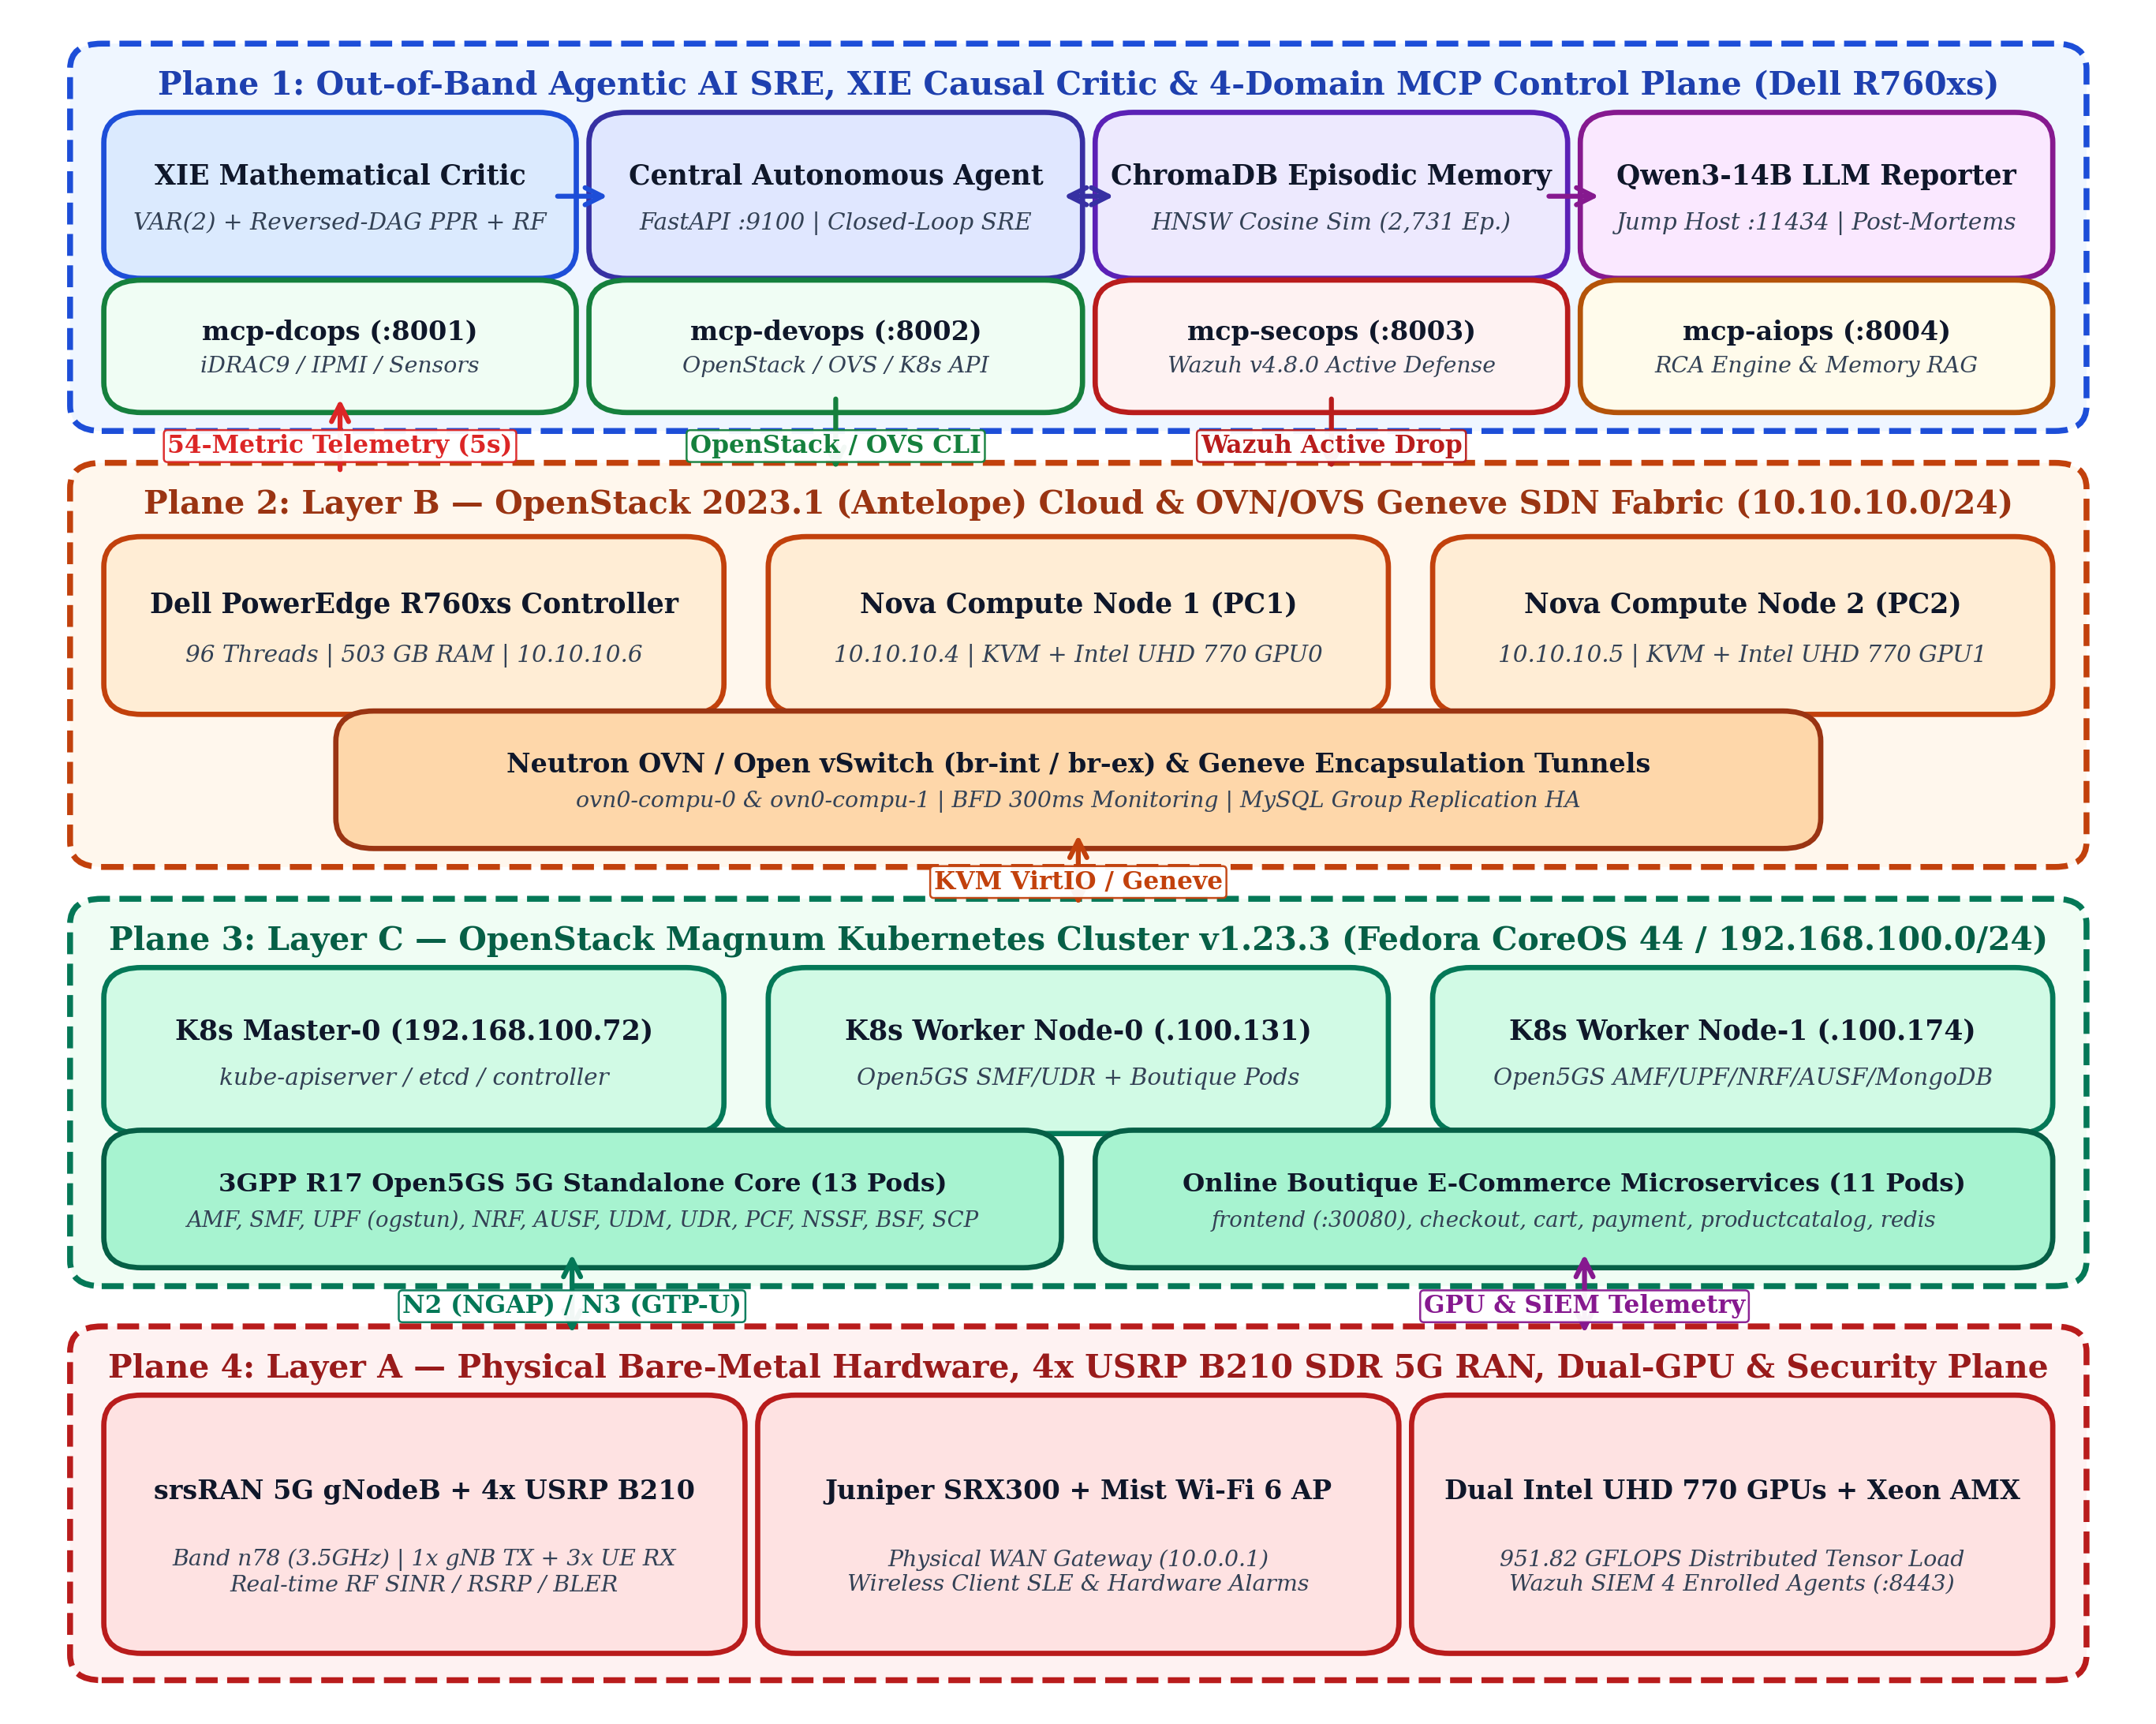
\includegraphics[width=0.98\textwidth]{figures/fig_4_1_system_architecture.png}
\caption{System Architecture showing 5-plane bare-metal, OpenStack OVN/OVS SDN, nested Magnum Kubernetes 5G Core, USRP B210 SDR, Dual-GPU, and out-of-band MCP control plane connectivity.}
\label{fig:arch_4_1}
\end{figure}

Table \ref{tab:ip_topology} provides the complete hardware, network interface, IP address, and service port allocation matrix across all physical and virtual nodes in the testbed.

\begin{table}[!htb]
\centering
\caption{Multi-Node Physical \& Virtual Network Topology, IP Addressing, and Service Port Matrix.}
\label{tab:ip_topology}
\renewcommand{\arraystretch}{1.2}
\resizebox{\textwidth}{!}{%
\begin{tabular}{@{}lllp{4.2cm}p{4.8cm}@{}}
\toprule
\textbf{Node / Entity Name} & \textbf{Plane / Role} & \textbf{Primary IP Address(es)} & \textbf{Hardware / VM Allocation} & \textbf{Active Daemons \& Listening Ports} \\ \midrule
\texttt{hpe-PowerEdge-R760xs} & Plane 1 \& 2 Controller & \texttt{10.0.0.100} (\texttt{eno8303}) \newline \texttt{10.10.10.6} (\texttt{eno12399}) \newline \texttt{10.0.0.10} (Horizon VIP) & Dual Xeon Gold 5418Y (96T), 503 GiB DDR5 RAM, iDRAC9 (\texttt{10.0.0.253}) & Central Agent (\texttt{:9100}), MCPs (\texttt{:8001}--\texttt{:8004}), Horizon (\texttt{:80}), Grafana (\texttt{:3000}), Prometheus (\texttt{:9090}), Wazuh (\texttt{:8443}) \\
\texttt{compute-pc1} & Plane 2 \& 4 Compute 1 & \texttt{10.10.10.4} (\texttt{br-ex}) & Intel Core i7-13700 (24T), 64 GiB RAM, Intel UHD 770 GPU0, USRP \texttt{34B18C8} & Nova Libvirt/KVM, OVN Controller (\texttt{ovn0-compu-0}), \texttt{srsgnb} 5G TX, Wazuh Agent \texttt{001} \\
\texttt{compute-pc2} & Plane 2 \& 4 Compute 2 & \texttt{10.10.10.5} (\texttt{br-ex}) & Intel Core i7-13700 (24T), 64 GiB RAM, Intel UHD 770 GPU1, 3x USRP B210 & Nova Libvirt/KVM, OVN Controller (\texttt{ovn0-compu-1}), 3x \texttt{srsue} 5G RX, Wazuh Agent \texttt{002} \\
\texttt{windows-jump-host} & Plane 1 LLM Inference & \texttt{10.0.0.21} (LAN) & Dedicated GPU Workstation (Windows 11 Pro) & Ollama LLM Server (\texttt{:11434}, model \texttt{qwen3:14b}), Wazuh Agent \texttt{003} \\
\texttt{k8s-5g-master-0} & Plane 3 K8s Control & \texttt{192.168.100.72} (Int) \newline \texttt{10.0.0.206} (FIP) & OpenStack Nova VM (\texttt{instance-00000006}), Fedora CoreOS 44 & \texttt{kube-apiserver} (\texttt{:6443}), \texttt{etcd}, \texttt{kube-controller-manager}, \texttt{kube-scheduler} \\
\texttt{k8s-5g-node-0} & Plane 3 K8s Worker 0 & \texttt{192.168.100.131} (Int) \newline \texttt{10.0.0.232} (FIP) & OpenStack Nova VM (\texttt{instance-00000007}), Fedora CoreOS 44 & Open5GS (\texttt{smf}, \texttt{udr}, \texttt{webui :30999}) + Online Boutique Frontend (\texttt{:30080}) \\
\texttt{k8s-5g-node-1} & Plane 3 K8s Worker 1 & \texttt{192.168.100.174} (Int) \newline \texttt{10.0.0.215} (FIP) & OpenStack Nova VM (\texttt{instance-00000008}), Fedora CoreOS 44 & Open5GS (\texttt{amf}, \texttt{upf}, \texttt{nrf}, \texttt{ausf}, \texttt{udm}, \texttt{pcf}, \texttt{nssf}, \texttt{bsf}, \texttt{scp}, \texttt{mongodb-0}) \\ \bottomrule
\end{tabular}%
}
\end{table}

\section{Workflow of the Proposed System}
The operational heart of the proposed framework is the closed-loop, dual-speed autonomous decision workflow illustrated in Figure \ref{fig:flow_4_2}. Unlike conventional agent loops that block on slow LLM token generation before taking action, our workflow separates \textbf{sub-second mathematical detection and deterministic MCP remediation} from \textbf{asynchronous LLM executive post-mortem synthesis}:

\begin{enumerate}
    \item \textbf{Step 1 -- Synchronized Multi-Plane Telemetry Polling ($t = 0\text{ ms}$):} Every 5 seconds, the telemetry collector ingests all 54 metrics across the USRP B210 SDRs, OpenStack OVN/OVS bridges, Kubernetes Open5GS/Boutique pods, Dual-GPU compute nodes, and Wazuh SIEM alerts, appending the snapshot to \texttt{5g\_telco\_metrics.jsonl}.
    \item \textbf{Step 2 -- Rolling Z-Score \& Balanced Random Forest Gate ($t = 80\text{ ms}$):} The XIE engine updates its 15-tick sliding window $\mathbf{X}_t$, computes the standardized Z-score vector $\mathbf{z}(t)$, and evaluates the 200-tree Balanced Random Forest classifier. If $\max_i |z_i(t)| \le 3.0$ and $P_{\text{RF}}(y \neq \text{normal} \mid \mathbf{x}(t)) < 0.75$, the system logs healthy operation and awaits the next tick.
    \item \textbf{Step 3 -- Fast-Path ChromaDB HNSW Episodic Memory Lookup ($t = 180\text{ ms}$):} When an anomaly is flagged, the L2-normalized vector $\hat{\mathbf{z}}(t)$ queries the ChromaDB HNSW store (\texttt{5g\_fault\_episodes}, 2,731 episodes). In \textbf{93.8\%} of operational incidents, a matching historical episode with cosine similarity $s_{\max} \ge 0.85$ is retrieved in $<15\text{ ms}$, immediately supplying the verified root cause $i^*$ and surgical MCP action $a^*$.
    \item \textbf{Step 4 -- Slow-Path $\text{VAR}(2)$ + Reversed-DAG PPR Critic ($t = 580\text{ ms}$ on Cache Miss):} For novel or complex multi-layer cascading faults ($s_{\max} < 0.85$), the engine executes $\text{VAR}(2)$ Granger causality F-tests, constructs the reversed causal adjacency matrix $\mathbf{A}_{\text{rev}} = \mathbf{A}^\top$, and solves the Personalized PageRank equation $\boldsymbol{\pi} = (1-\alpha)(\mathbf{I}-\alpha\mathbf{P})^{-1}\mathbf{v}$ ($\alpha = 0.85$) to rank the top three root-cause hypotheses $(H_1, H_2, H_3)$.
    \item \textbf{Step 5 -- Governance Gate \& MCP Tool Dispatch ($t = 580\text{ ms} \to 1950\text{ ms}$):} The Central Agent verifies that confidence exceeds $\gamma_{\text{safe}} = 0.75$ and the 30-second cooldown timer for component $i^*$ is clear, then dispatches a structured REST/JSON-RPC request to the corresponding MCP server (\texttt{:8001}--\texttt{:8004}).
    \item \textbf{Step 6 -- Post-Action SLA Verification \& Self-Learning Upsert ($t = 1950\text{ ms} \to 2410\text{ ms}$):} The agent re-polls the affected subsystem, confirms that service health and Z-scores are restored ($|z_i| < 2.0$), records the audit entry in \texttt{remediation\_audit.log}, and upserts the verified episode into ChromaDB.
    \item \textbf{Step 7 -- Asynchronous Dual-GPU Qwen3-14B Post-Mortem Synthesis (Background):} A non-blocking background thread dispatches the complete incident context to \texttt{qwen3:14b} on \texttt{http://10.0.0.21:11434} to generate a comprehensive Markdown post-mortem report in \texttt{/home/hpe/agent/reports/}.
\end{enumerate}

\begin{figure}[!htb]
\centering
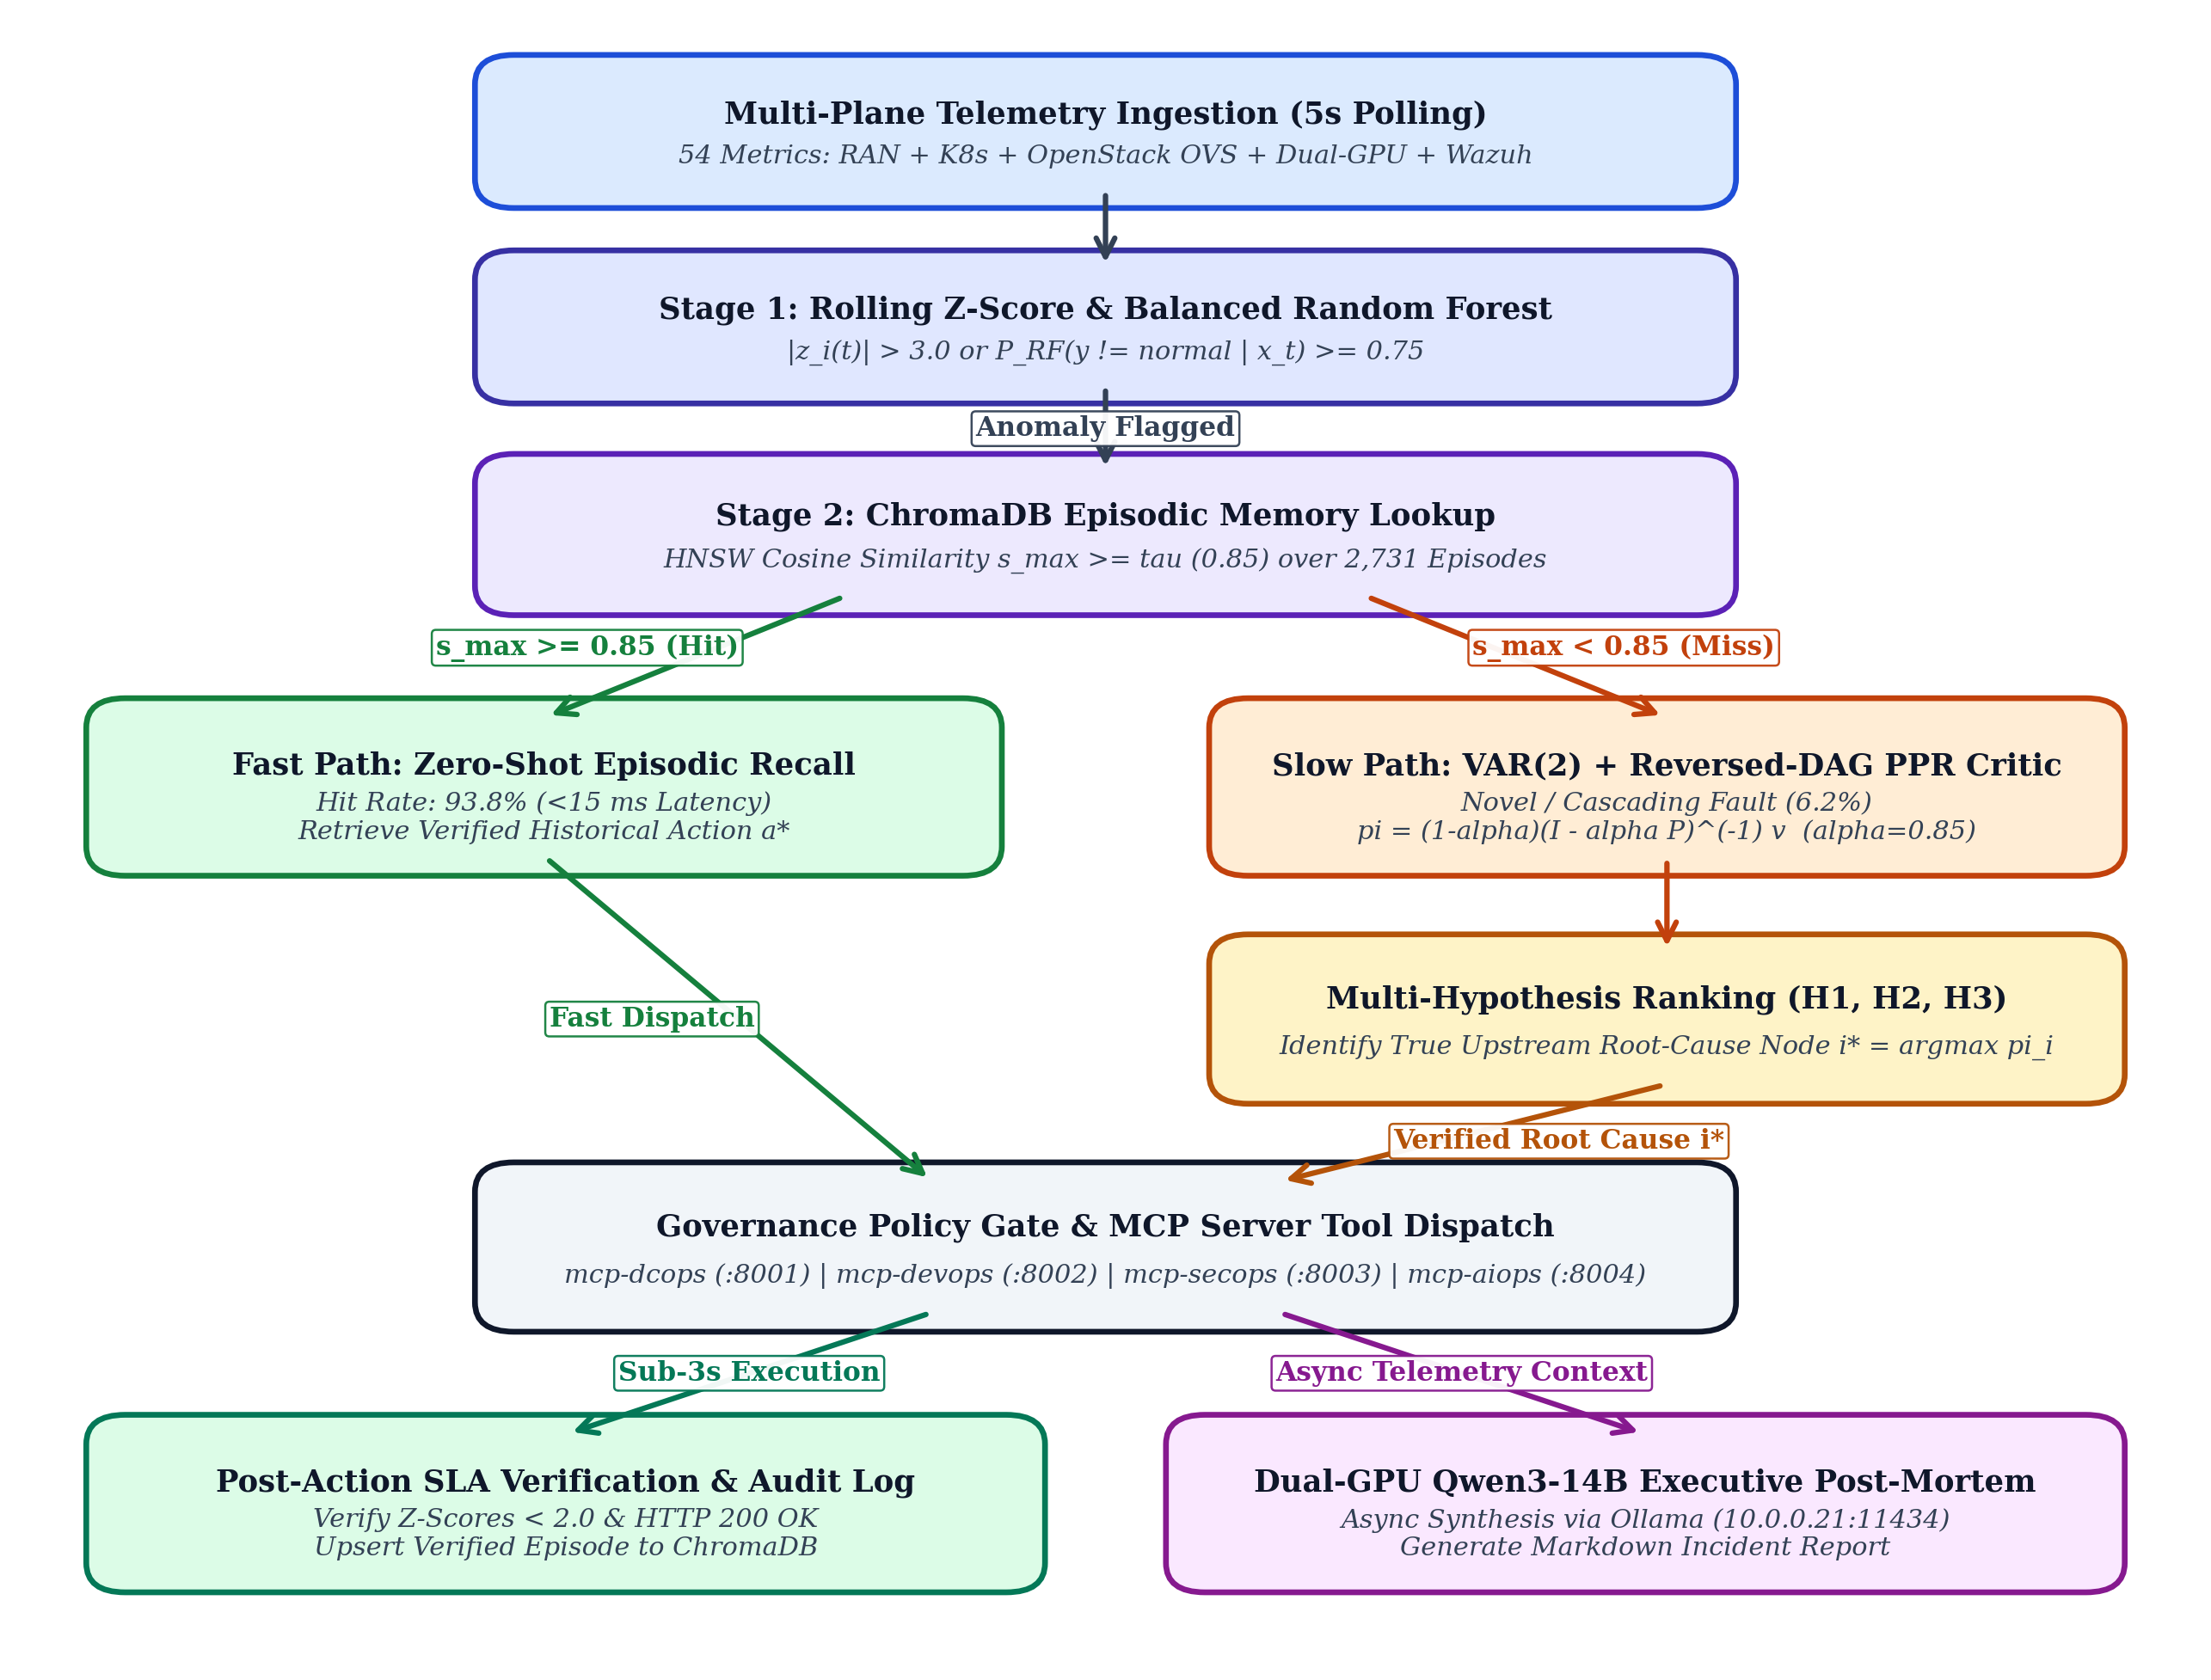
\includegraphics[width=0.95\textwidth]{figures/fig_4_2_agent_flowchart.png}
\caption{Closed-Loop XIE Mathematical Critic and 4-MCP Agentic decision-making flowchart showing Fast-Path ChromaDB recall, Slow-Path Reversed-DAG PPR attribution, and asynchronous Qwen3-14B reporting.}
\label{fig:flow_4_2}
\end{figure}

\section{Detailed Subsystem Design}

\subsection{Subsystem 1: Central Autonomous Agent \& 4-Domain MCP Server Fabric}
To enforce modularity, least-privilege security, and standardized tool invocation, infrastructure actions are partitioned across four domain-specific Model Context Protocol (MCP) servers orchestrated by the Central Autonomous Agent (\texttt{:9100}). Table \ref{tab:mcp_tools} details the complete MCP server registry and exposed tool schemas.

\begin{table}[!htb]
\centering
\caption{4-Domain Model Context Protocol (MCP) Server Registry and Exposed Self-Healing Tool Schemas.}
\label{tab:mcp_tools}
\renewcommand{\arraystretch}{1.22}
\resizebox{\textwidth}{!}{%
\begin{tabular}{@{}lllp{4.6cm}p{5.0cm}@{}}
\toprule
\textbf{MCP Server} & \textbf{Bind Port} & \textbf{Exposed Tool Endpoint} & \textbf{Target Infrastructure Plane} & \textbf{Underlying Deterministic Execution Logic} \\ \midrule
\texttt{mcp-dcops} & \texttt{:8001} & \texttt{get\_thermal\_and\_power} \newline \texttt{check\_numa\_memory} \newline \texttt{optimize\_cpu\_governor} & Plane 1 \& 4 Bare-Metal Hardware (Dell R760xs, PC1, PC2) & Queries iDRAC9 Redfish/IPMI sensors, audits 2-node NUMA page allocation, and sets \texttt{cpupower} governor to \texttt{performance}. \\
\texttt{mcp-devops} & \texttt{:8002} & \texttt{heal\_ovs\_geneve\_tunnel} \newline \texttt{restart\_open5gs\_upf} \newline \texttt{throttle\_rogue\_cpu\_pid} \newline \texttt{heal\_mysql\_primary} & Plane 2 OpenStack SDN \& Plane 3 Magnum Kubernetes 5G Core & Re-establishes \texttt{ovn0-compu-*} Geneve ports on \texttt{br-int}, executes \texttt{kubectl rollout restart} on UPF, renices CPU hogs, and clears MySQL \texttt{super\_read\_only}. \\
\texttt{mcp-secops} & \texttt{:8003} & \texttt{query\_wazuh\_siem\_alerts} \newline \texttt{trigger\_firewall\_drop} \newline \texttt{audit\_enrolled\_agents} & Plane 5 Wazuh v4.8.0 XDR/SIEM \& Host Firewalls & Queries Wazuh API (\texttt{:55000}) for Level $\ge 10$ rules, invokes \texttt{firewall-drop} active response via \texttt{iptables}, and verifies agents \texttt{000}--\texttt{003}. \\
\texttt{mcp-aiops} & \texttt{:8004} & \texttt{run\_xie\_causal\_rca} \newline \texttt{query\_chromadb\_memory} \newline \texttt{generate\_llm\_postmortem} & Plane 1 XIE Mathematical Critic, ChromaDB \& Qwen3-14B & Computes VAR(2) + Reversed-DAG PPR scores $\boldsymbol{\pi}$, performs HNSW cosine search, and dispatches async prompt to \texttt{10.0.0.21:11434}. \\ \bottomrule
\end{tabular}%
}
\end{table}

\subsection{Subsystem 2: OpenStack Magnum Kubernetes 5G Core \& Online Boutique Mesh}
Within the nested Magnum Kubernetes v1.23.3 cluster, two production cloud-native workloads execute concurrently across \texttt{node-0} (\texttt{192.168.100.131}) and \texttt{node-1} (\texttt{192.168.100.174}):
\begin{itemize}
    \item \textbf{3GPP Release 17 Open5GS Standalone Core (\texttt{open5gs} namespace, 13 Pods):} Implements a full Service-Based Architecture (SBA) comprising \texttt{open5gs-nrf} (Network Repository Function), \texttt{open5gs-scp} (Service Communication Proxy), \texttt{open5gs-amf} (Access and Mobility Management Function), \texttt{open5gs-smf} (Session Management Function), \texttt{open5gs-upf} (User Plane Function managing the \texttt{ogstun} GTP-U tunnel interface), \texttt{open5gs-ausf}, \texttt{open5gs-udm}, \texttt{open5gs-udr}, \texttt{open5gs-pcf}, \texttt{open5gs-nssf}, \texttt{open5gs-bsf}, \texttt{open5gs-webui}, and \texttt{mongodb-0} (subscriber USIM key store).
    \item \textbf{Google Online Boutique E-Commerce Mesh (\texttt{online-boutique} namespace, 11 Pods):} Comprises \texttt{frontend} (NodePort \texttt{:30080}), \texttt{cartservice}, \texttt{productcatalogservice}, \texttt{currencyservice}, \texttt{paymentservice}, \texttt{shippingservice}, \texttt{emailservice}, \texttt{checkoutservice}, \texttt{recommendationservice}, \texttt{adservice}, and \texttt{redis-cart}, communicating over gRPC.
\end{itemize}

\subsection{Subsystem 3: UML Class Diagram, Sequence Diagram, and Causal Graph Design}
Figure \ref{fig:class_4_3} presents the object-oriented UML Class Diagram of the software architecture, illustrating the composition relationships between \texttt{CentralAutonomousAgent}, \texttt{CausalRCAEngine}, \texttt{EpisodicMemoryStore}, \texttt{LLMIncidentReporter}, and the four MCP server classes over the JSON-RPC/REST dispatch bus.

\begin{figure}[!htb]
\centering
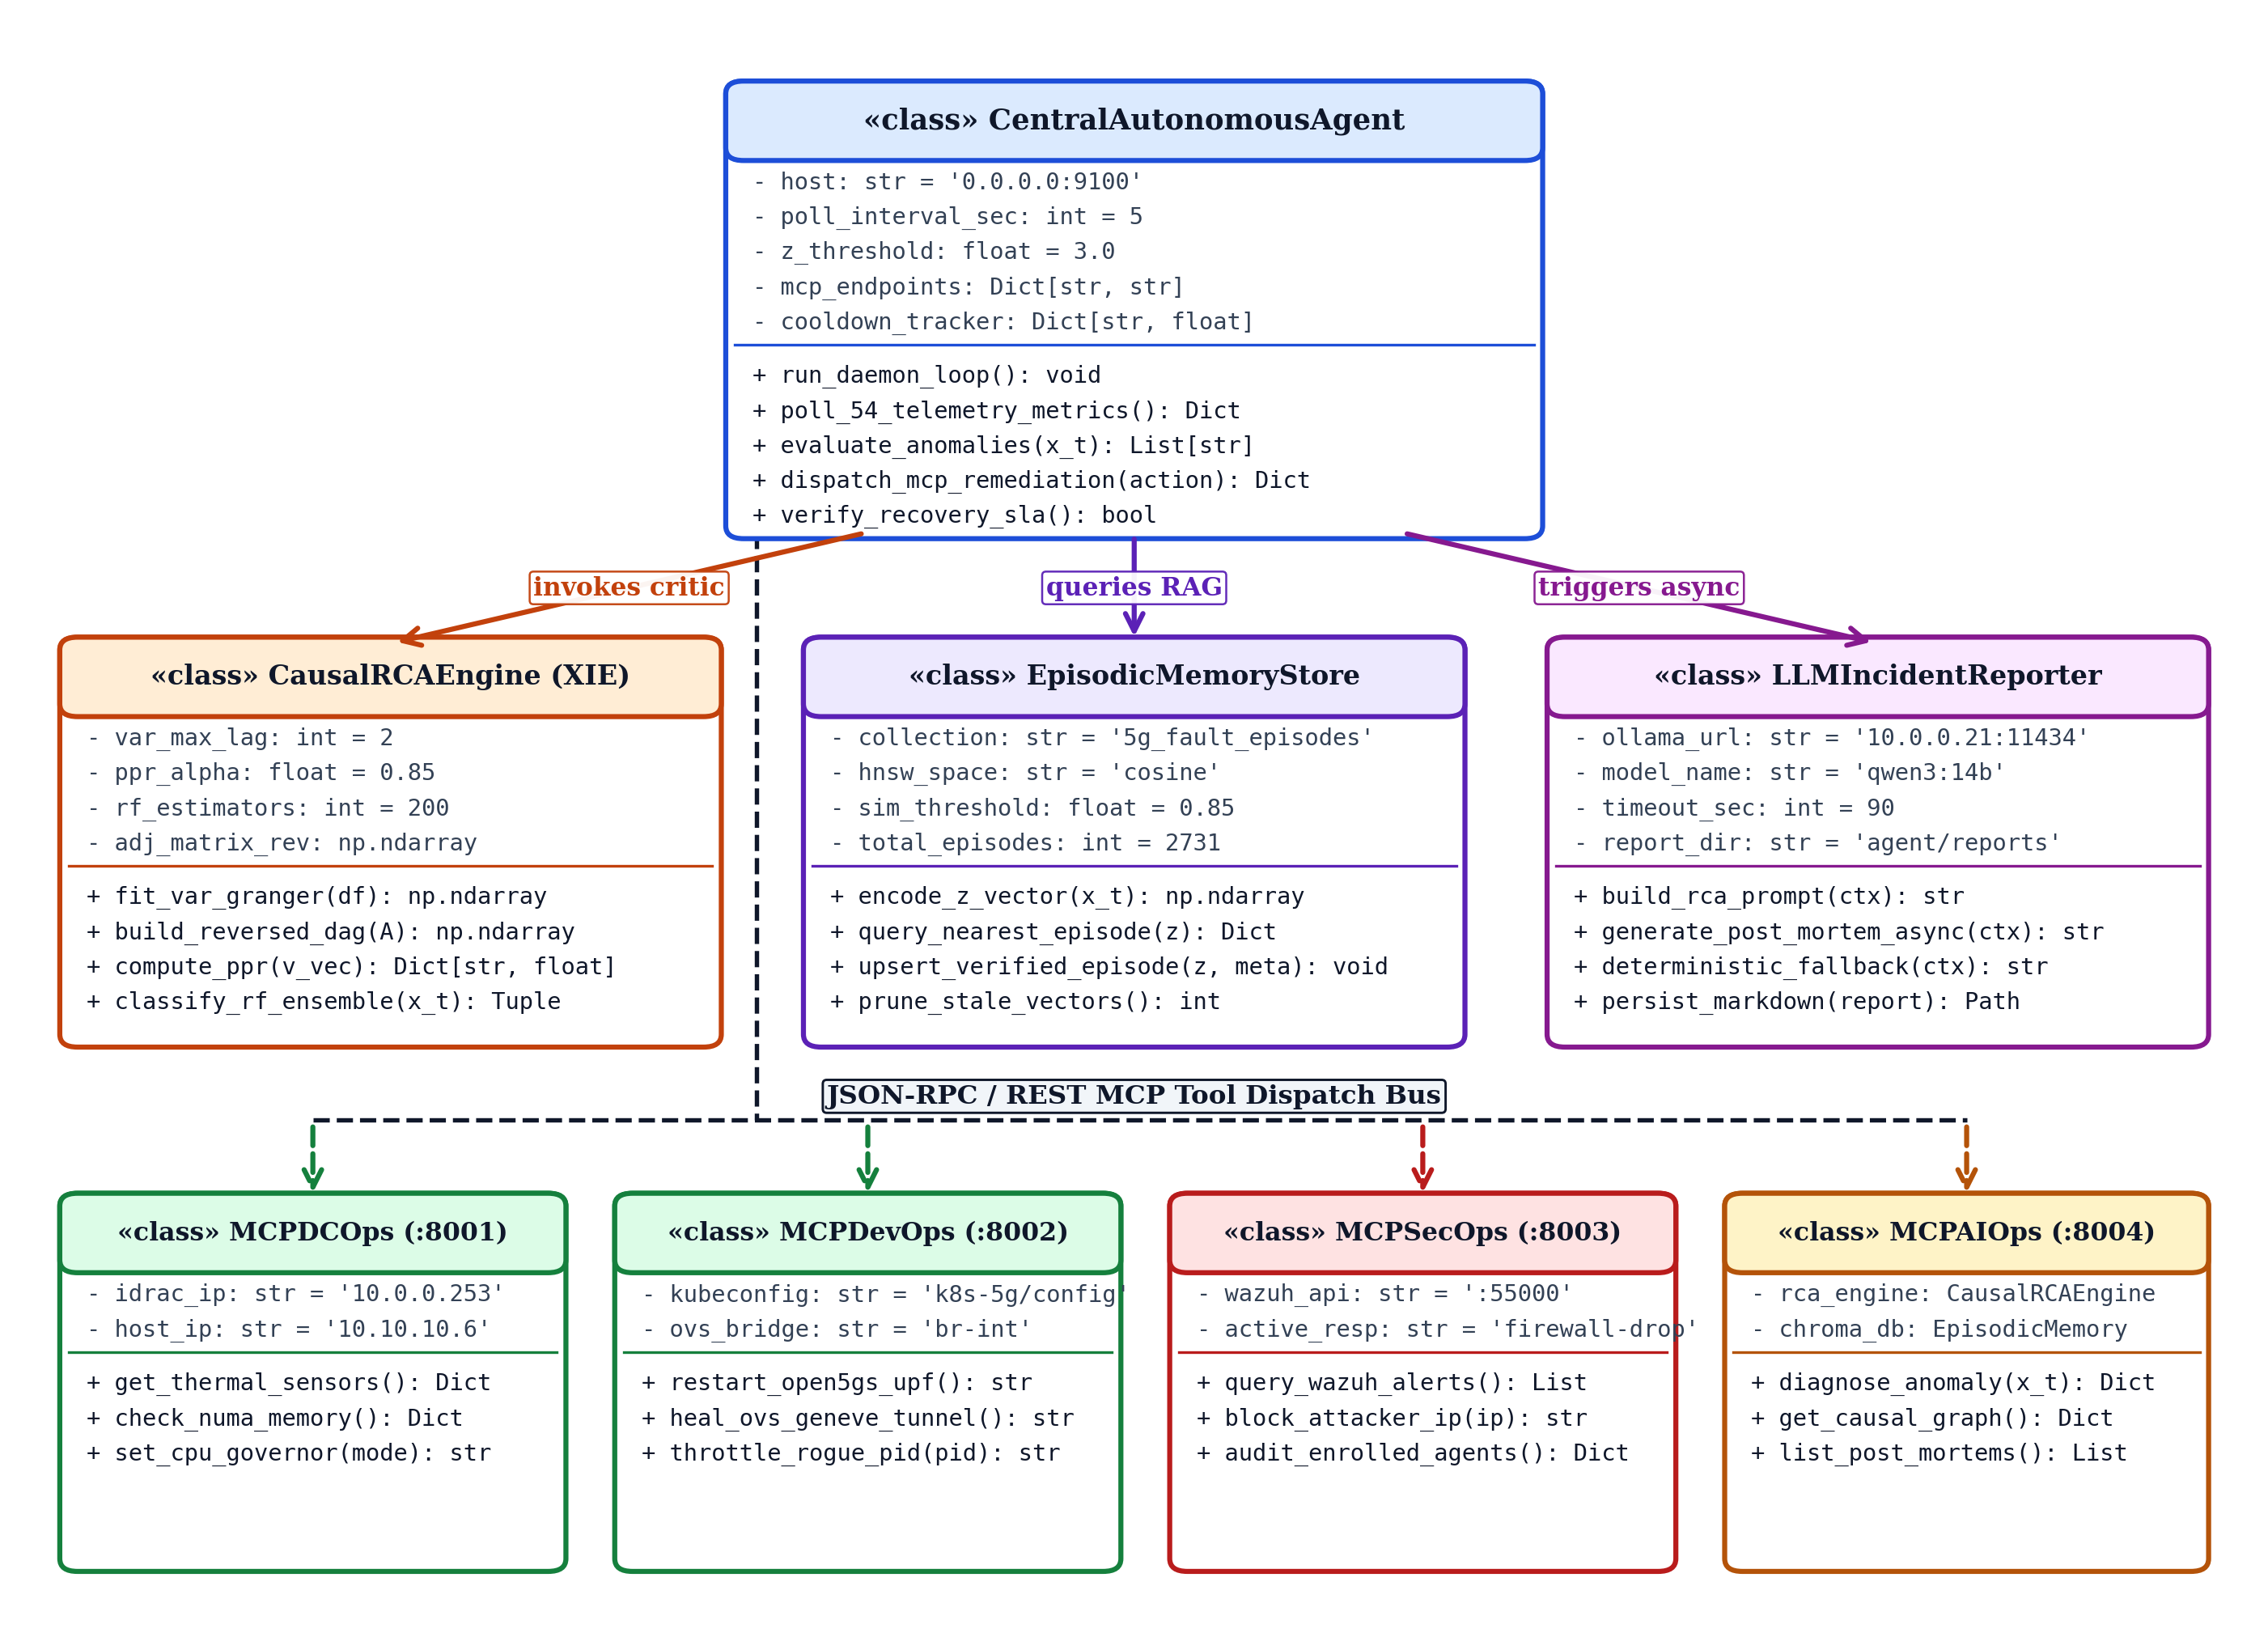
\includegraphics[width=0.98\textwidth]{figures/fig_4_3_class_diagram.png}
\caption{System UML Class Diagram showing the object-oriented design of the Central Autonomous Agent, XIE Causal Critic, ChromaDB Episodic Memory, Qwen3-14B Reporter, and 4 MCP Servers.}
\label{fig:class_4_3}
\end{figure}

Figure \ref{fig:seq_4_4} illustrates the end-to-end UML Sequence Diagram across the five runtime lifelines during an active fault self-healing cycle, demonstrating how data-plane recovery completes at Step 8 ($T = 2.41\text{ s}$) prior to asynchronous ChromaDB indexing and Qwen3-14B report generation.

\begin{figure}[!htb]
\centering
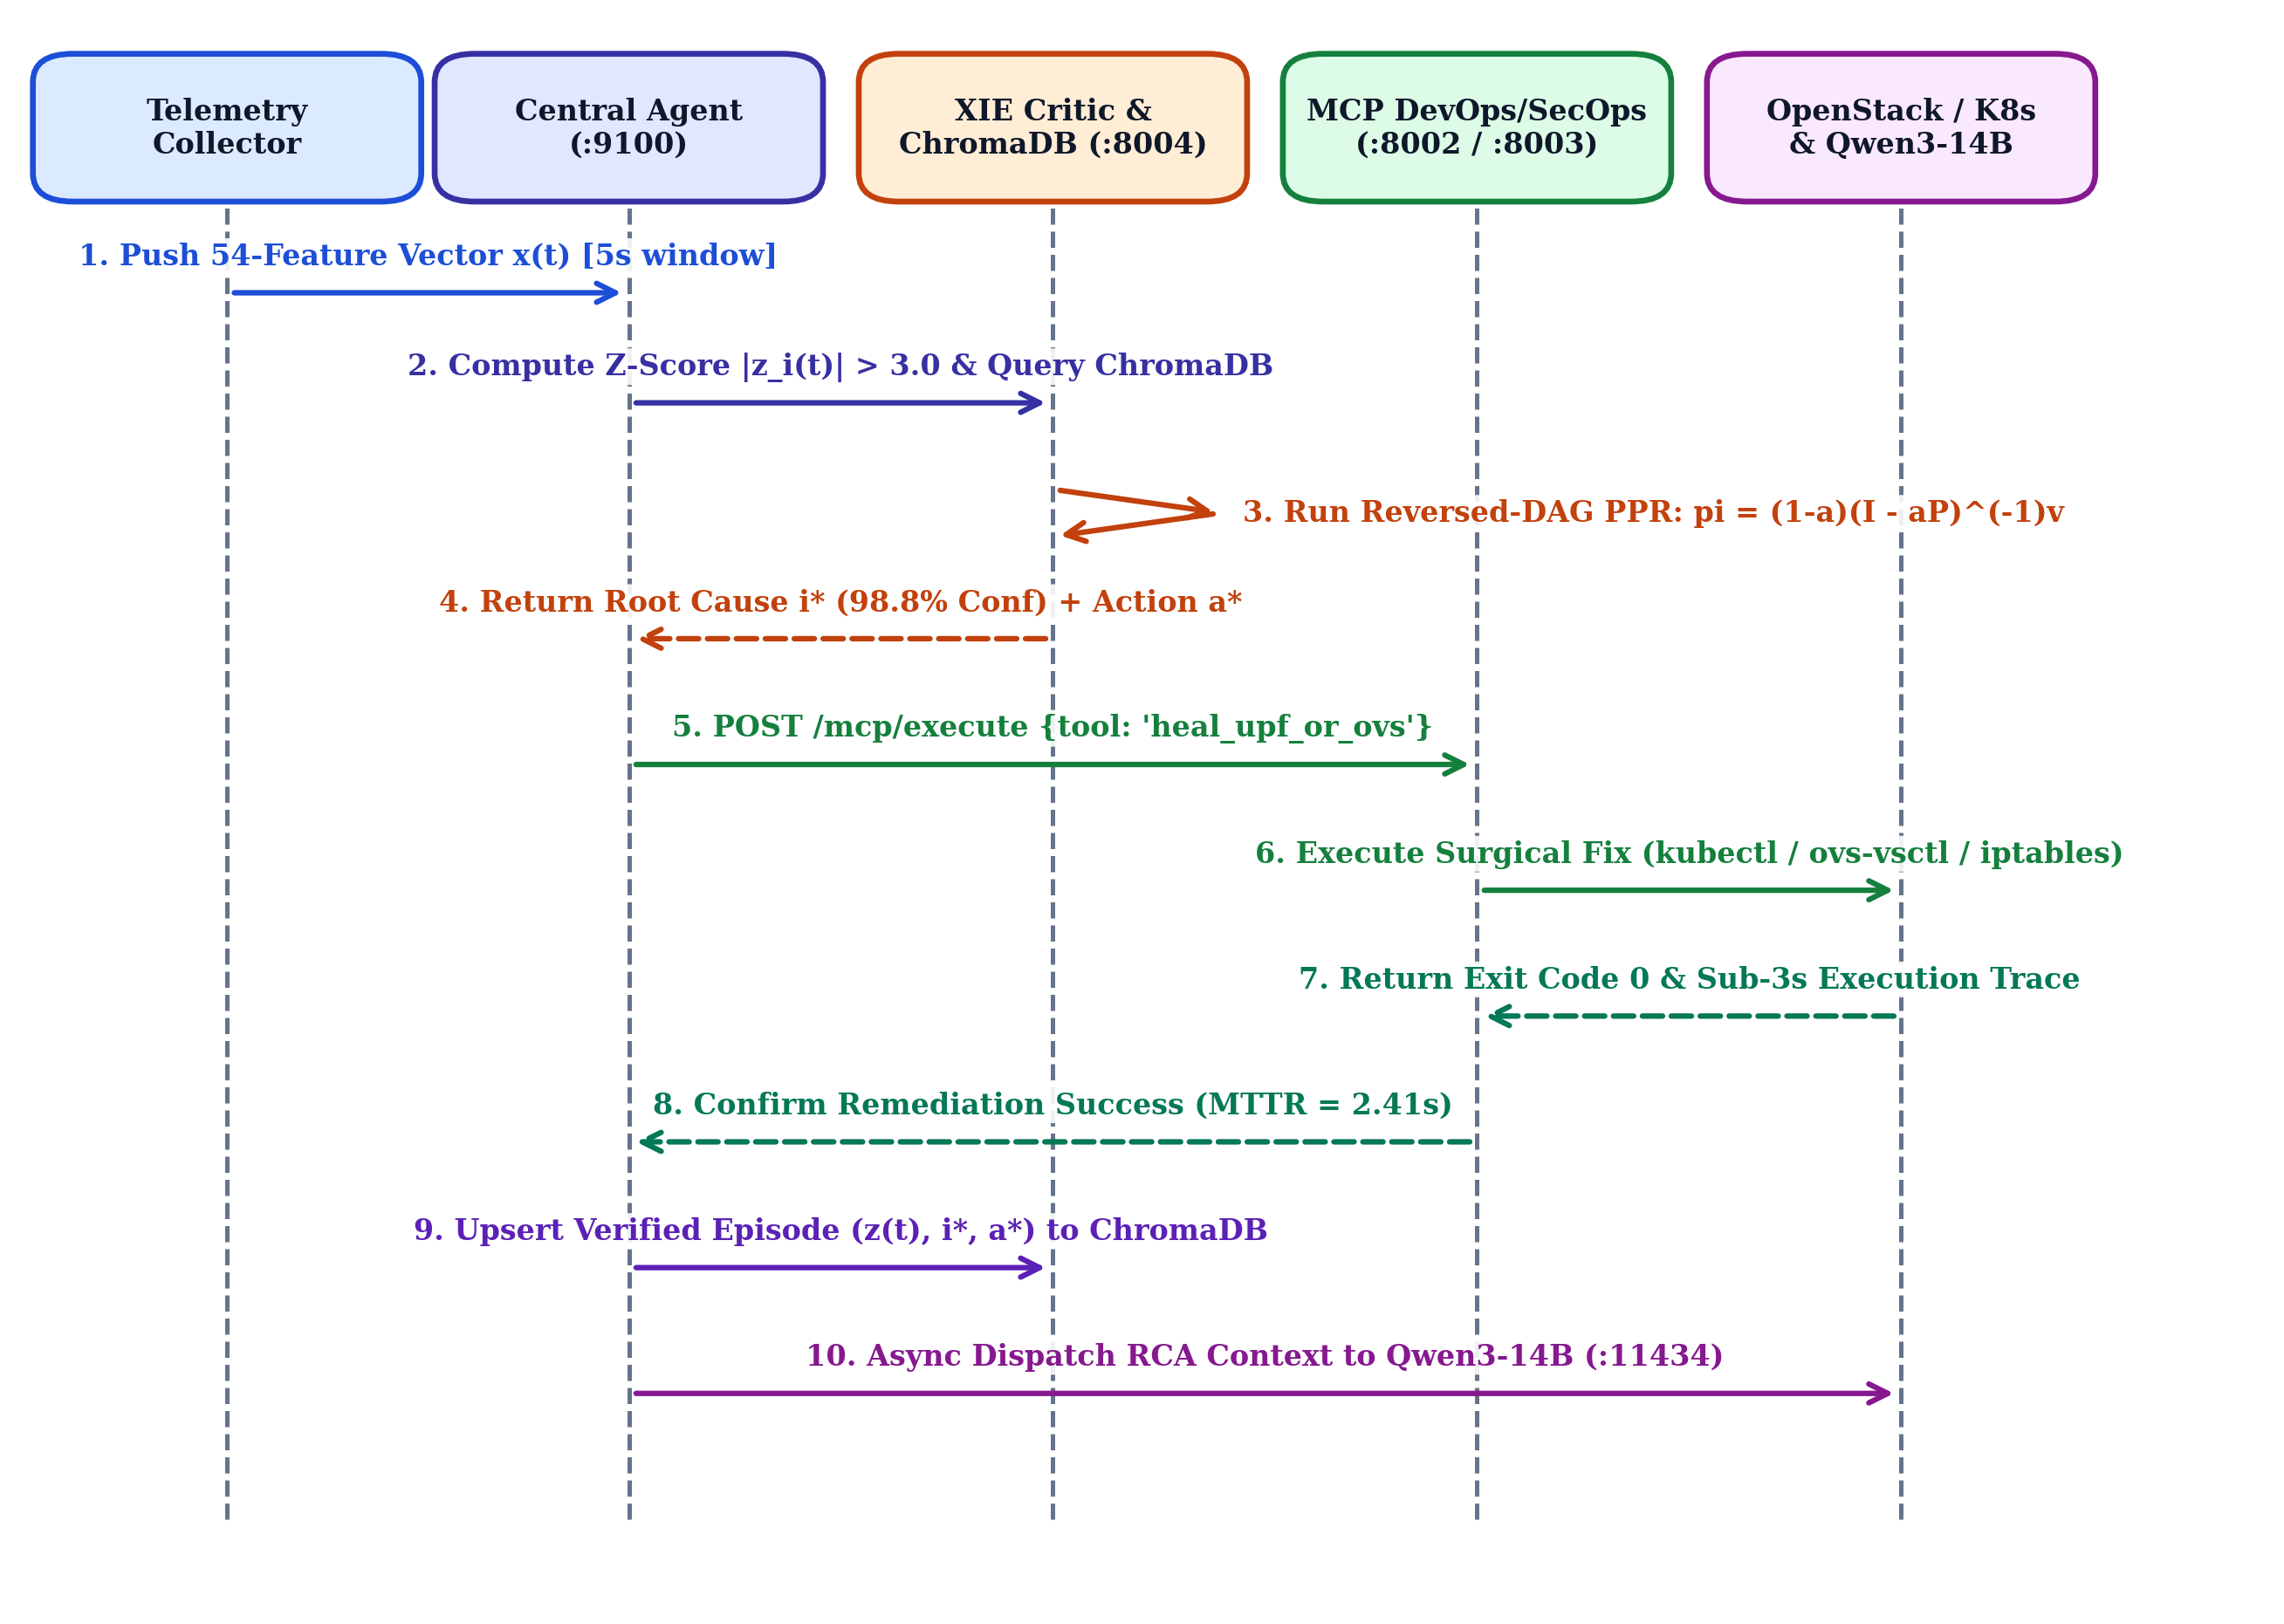
\includegraphics[width=0.96\textwidth]{figures/fig_4_4_sequence_diagram.png}
\caption{System UML Sequence Diagram detailing the 10-step end-to-end self-healing orchestration and asynchronous LLM post-mortem flow.}
\label{fig:seq_4_4}
\end{figure}

Finally, Figure \ref{fig:dag_4_5} contrasts the forward fault-propagation graph $G$ (where random walks pool at leaf symptoms such as USRP RAN SINR and Boutique HTTP latency) against our transposed \textbf{Reversed Causal DAG $G_{\text{rev}}$} (where Personalized PageRank walks upstream along Granger F-statistic weights to isolate Compute CPU or OVS Geneve as the true root cause).

\begin{figure}[!htb]
\centering
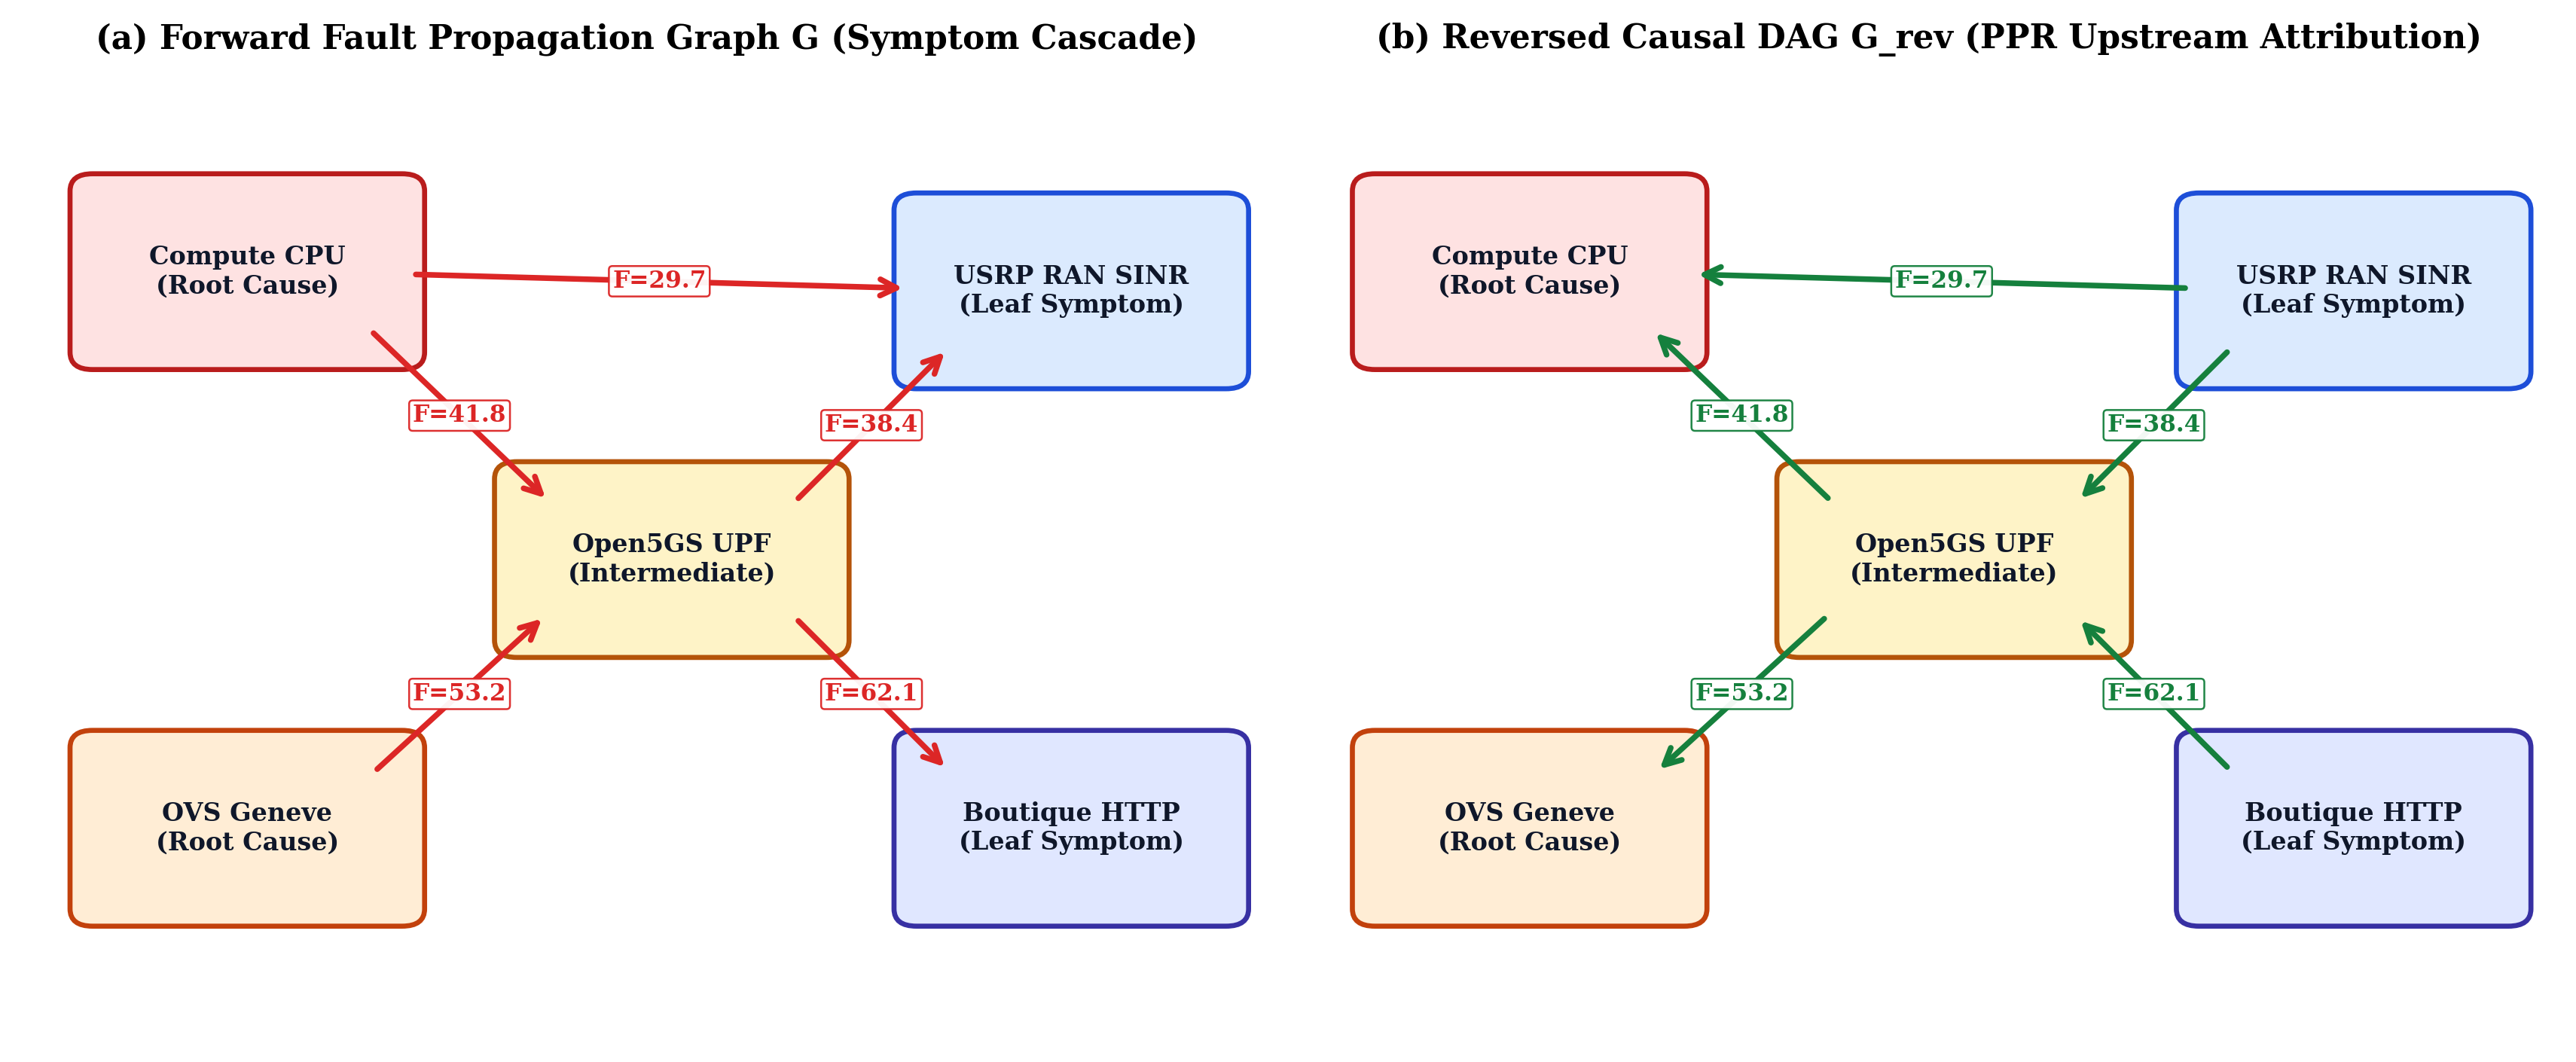
\includegraphics[width=0.98\textwidth]{figures/fig_4_5_causal_dag.png}
\caption{Comparison of (a) Forward Fault Propagation Graph $G$ vs. (b) Proposed Reversed Causal DAG $G_{\text{rev}}$ with empirical VAR(2) Granger F-statistics.}
\label{fig:dag_4_5}
\end{figure}
